\chapter{Concurrent CertiKOS Framework}
\label{chap:con}

In this chapter, we will show how to
extend the sequential \CTOS{} framework
with the global log
to support concurrent program reasoning.
Section~\ref{sec:layer} introduces
the concurrent abstract machine with
global log, which extends the layer calculus
to support concurrent abstraction layers.
In Section~\ref{sec:mach},
we show a chain of concurrent
machine models from
multicore hardware machine
to a CPU-local machine.
Therefore,  most of the concurrent code
can be verified similar to sequential code,
making it possible to reuse lots of tools
developed in the sequential \CTOS{} framework.
\ignore{In Section~\ref{sec:comp},
we show how to equip CompCertX
with algebraic memory model to form a verified \emph{thread-safe} C compiler.}

%\section{Informal Development}
\label{sec:informal}

In this section, we give an overview of a few high-level ideas on how
we build certified concurrent layers. 

Like a sequential layer~\cite{dscal15}, each concurrent layer can also
contain thread-private abstract states (refined from the concrete
thread-local in-memory data) and related abstract primitives. However,
the data shared by multiple threads are not represented as abstract
states. Instead, each method call to a shared atomic object is
recorded as an observable event and is appended to the end of a shared
global log. For each shared object, we define a {\em replay} function
that can reconstruct the current shared state from the current global
log. Thus, all shared objects are represented as a single sequence of
logged events with appropriate replay functions.

With concurrency, the machine semantics for each layer (e.g.,
$\sem{L}{\cdot}$) is no longer deterministic: for each scheduler
strategy ($\strat{hs}$), it may generate a different global
log. To prove the simulation $\sem{L'}{P\oplus{}M} \leq_R \sem{L}{P}$,
for each scheduler strategy $\strat{hs}$, if running $P\oplus{}M$ on
machine $L'$ with $\strat{hs}$ produces a global log $l$, we must find
another scheduler strategy $\stratp{hs}$ such that running $P$ on
machine $L$ under $\stratp{hs}$ would generate a global log $l'$ that
is related to $l$ via the simulation relation $R$. We will actually
construct a {\em function} that will map $l$ and $\strat{hs}$ into
$l'$ and $\stratp{hs}$. Of course, the simulation relation $R$ over
thread-private states might still be a relation~\cite{dscal15}.

\paragraph{An example of concurrent layers}
The example in Figure~\ref{fig:exp:ticket_lock_example} contains a
client program $P$ which has two threads running on two different
CPUs; each thread makes one call to the atomic primitive $\comm{foo}$
provided by the layer interface $L_3$.

Concurrent object module $M_2$ implements the layer interface $L_3$
but it is built on top of $L_2$.  The $\comm{foo}$ method calls two
atomic primitives $f$ and $g$ in a critical section protected by a
ticket lock~\cite{mcs91}.

%%%%%%%%%%%%%%%%%%%%%%%%%%%%%%
\begin{figure}
\lstinputlisting [language = C, multicols=2] {source_code/ticket_lock_example.c}
%\vspace{-5pt}
\caption{Building certified concurrent layers over a ticket lock}
\label{fig:exp:ticket_lock_example}
\vspace{-10pt}
\end{figure}
%%%%%%%%%%%%%%%%%%%%%%%%%%%%%%

The ticket-lock module $M_1$ is built on top of $L_1$ and it
implements $L_2$. Even though the implementation of a ticket lock
contains two shared integer value fields: $\comm{ticket}$ and
$\comm{now}$ (where $\comm{now} \leq \comm{ticket}$ always holds), the
interface $L_1$ only provides the atomic primitives such as
fetch-and-incrementing the $\comm{ticket}$ value, getting the current
$\comm{now}$ value, holding the lock (if the $\comm{now}$ value is
equal to the $\comm{ticket}$ value), and incrementing the $\comm{now}$
value (to release the lock). The current $\comm{ticket}$ and
$\comm{now}$ values can be reconstructed by replaying the global log
(for the $L_1$ machine).  $L_1$ also provides the atomic $\comm{f}$
and $\comm{g}$ events which are later passed on to $L_2$.

\paragraph{Strategy, environment context, and layer simulation}
Our goal is to show that for each run of $P\oplus{}M_2\oplus{}M_1$
over $L_1$, we can find another run of $P$ over $L_3$ so that the
global logs produced by both runs are related.
To show how we accomplish this, here is
a global log $l_{g1}$ produced from  
a specific run of $P\oplus{}M_2\oplus{}M_1$ over $L_1$.

\vspace*{-1ex}
% \colorbox{Peach}{\textcolor{white}{a}}
\begin{small}
\[
\begin{array}{l}
\ssame \cons (1.\incticket) \cons
\sdiff \cons (2.\incticket) \cons
\ssame \cons (2.\getnow) \cons
\sdiff \cons (1.\getnow) \cons
\ssame \cons (1.\holdlock) 
\\
\cons 
\sdiff \cons (2.\getnow) \cons
\sdiff \cons (1.\comm{f}) \cons
\sdiff \cons (2.\getnow) \cons
\sdiff \cons (1.\comm{g}) \cons
\ssame \cons (1.\incnow) 
\\
\cons \sdiff \cons (2.\getnow) \cons
\ssame \cons (2.\holdlock) \cons
\ssame \cons (2.\comm{f}) \cons
\ssame \cons (2.\comm{g}) \cons
\ssame \cons (2.\incnow) 
\end{array}
\]
\end{small}%

Throughout this paper, we assume that all programs always
start from CPU 1, and before each CPU executes an atomic primitive,
it always yields to the hardware scheduler ($hs$).
We use $\ssame$ to denote a hardware yield to the same CPU,
and $\sdiff$ for a yield to a different CPU; each such symbol
is actually an abbreviation of two consecutive switch events: switch
from CPU $i$ to $hs$ (\ie, $i\switch{}hs$), and then switch from $hs$
to CPU $j$ (\ie, $hs \switch j$).  For example, starting from CPU 1,
$\sdiff$ is an abbreviation of $(1\switch{}hs) \cons (hs\switch 2)$.

We define $\comm{target}(l)$ as the switching destination of the last event in
the log $l$, which can be either 1, 2, or $hs$. The above run,
which produced the global log $l_{g1}$, can be viewed as combining
the following {\em strategies} defined for each CPU and $hs$:

\vspace*{-1ex}
\begin{small}
\[
\strat{j} (l)=
\begin{cases}
  j.e & \text{if } (\comm{target}(l) = j) ~~\wedge \\
      & ~~~~~(l\cons (j.e)) |_{j,hs} \text{ is a prefix of } (l_{g1} |_{j,hs}) \\
\comm{undefined } & \text{otherwise}
\end{cases}
\]
\end{small}%

\noindent{}Here, $l |_{j,hs}$ only keeps those events in $l$ that are
related to participants $j$ and $hs$.  For the hardware scheduler's
strategy $\strat{hs}$, this filtering essentially means that
regardless how the CPUs (or threads) are going to play in the interim,
$hs$'s moves will always follow $l_{g1}$.  Because $\strat{hs}$
defines how switching between different CPUs is done, when we define
each CPU's strategy, we filter out other CPUs' events but still keep
those events related to $hs$.

At each step, depending on the destination ($j$) of the current log
($l$), we can query the corresponding strategy $\strat{j}(l)$ to get the
next move for $j$.  For example, if the destination is $hs$, that is,
the log ends with $(\any\switch hs)$, then it is the
hardware scheduler's turn to generate a switch event $(hs\switch \any)$.

These strategies also form a nice decomposition of the global log
$l_{g1}$. To reason about CPU 1 alone, we only need to construct
its environment context $\oracle_1 := \strat{hs} \bigcup \strat{2}$.

The layer interface $L_2$ introduces the $\acq$ and $\rel$ primitives
which trigger events $\acq$ and $\rel$ respectively. Running
$P\oplus{}M_2$ over $L_2$ could produce the following shared log $l_{g2}$:

\vspace*{-1ex}
\begin{small}
\[
\begin{array}{l}
\ssame \cons (1.\acq) \cons
\ssame \cons (1.\comm{f}) \cons
\ssame \cons (1.\comm{g}) \cons
\ssame \cons (1.\rel) 
\\
\cons \sdiff \cons (2.\acq) \cons
\ssame \cons (2.\comm{f}) \cons
\ssame \cons (2.\comm{g}) \cons
\ssame \cons (2.\rel) 
\end{array}
\]
\vspace{-5pt}
\end{small}%

The layer interface $L_3$ introduces the atomic $\comm{foo}$
primitive. Running $P$ over $L_3$ could produce the following shared log
$l_{g3}$:
\vspace*{-1ex}
\begin{small}
\[
\ssame \cons (1.\comm{foo})
\cons \sdiff \cons (2.\comm{foo})
\]
\vspace{-7pt}
\end{small}%

To build a simulation, we want to define a function mapping one
layer's log and environment context into those of another layer.  For
example, the function $f_l$, mapping a log over $L_1$ into one over
$L_2$, can be defined as follows: (1) it maps the $\holdlock$ and
$\incnow$ events in $L_1$ to $\acq$ and $\rel$ events in $L_2$; (2) it
drops the $\incticket$ and $\getnow$ events; 
and (3) it merges all the adjacent switch symbols (\eg,
$\ssame \cons \sdiff$ is merged into $\sdiff$).
The following shows that $l_{g2} = f_l (l_{g1})$ is true:

\vspace*{-1ex}
\begin{small}
\[
\begin{array}{l}
\hspace*{-1em}\mysout
{\ssame \cons (1.\incticket) \cons
\sdiff \cons (2.\incticket) \cons
\ssame \cons (2.\getnow) \cons
\sdiff \cons (1.\getnow) \cons
}
\ssame \cons (1.\cancel{\holdlock}/\acq) 
\\
\hspace*{-1em}\mysout
{\cons 
\sdiff \cons (2.\getnow) \cons
\sdiff 
} 
\ssame \cons (1.\comm{f}) \cons
\mysout
{\sdiff \cons (2.\getnow) \cons
\sdiff
}
\ssame \cons (1.\comm{g}) \cons
\ssame \cons (1.\cancel{\incnow}/\rel) 
\\
\hspace*{-1em}\cons \sdiff 
\mysout
{\cons (2.\getnow) \cons
\ssame 
}
\cons (2.\cancel{\holdlock}/\acq) \cons
\ssame \cons (2.\comm{f}) \cons
\ssame \cons (2.\comm{g}) \cons
\ssame \cons (2.\cancel{\incnow}/\rel) 
\end{array}
\]
\end{small}

From $f_l$, we can construct a function $f_{\strat{}}$
that maps each strategy $\strat{j}$ for $L_1$ into one for $L_2$:

\vspace*{-1ex}
\begin{small}
\[ 
f_{\strat{}}(\strat{j}) (l'')=
\begin{cases}
j.e' & \text{if } 
\exists l', f_l(l') = l'' \wedge \strat{j}(l') = j.e\\
&\qquad\ \wedge f_l(l'\cons(j.e)) = l'' \cons (j.e') \\
\comm{undefined } & \text{otherwise}
\end{cases}
\]
\end{small}

Here, since many $L_1$ events are dropped in $L_2$,
the $L_2$ strategy $f_{\strat{}}(\strat{j})$ for $j$
has to keep querying $\strat{j}$ until
it also returns an event from $j$ at $L_2$.  For example, let $l'$ be
$\ssame \cons (1.\incticket) \cons \sdiff \cons (2.\incticket) \cons
\ssame \cons (2.\getnow) \cons \sdiff \cons (1.\getnow) \cons \ssame$,
since $\strat{1} (l') = 1.\holdlock$ and $f_l(l') = \ssame$, we have
$f_{\strat{}}(\strat{1}) (\ssame) =1.\holdlock$.

Finally, from $f_{\strat{}}$ we can construct the function
$f_{\oracle}$ which will map each environment context $\oracle$ for
$L_1$ into one for $L_2$.

\paragraph{Layer verification and composition}
Reasoning about a concrete strategy is simple, but when we verify
a concurrent module, we cannot assume such a specific environment context.
Instead, to verify
a layer running on CPU~$i$, we have to show that its implementation
meets its specification for all possible environment contexts
$\oracle_i$ that satisfy its ``rely'' invariants.

For example, to show that $\ltyp{L_1[1]}{R}{M_1}{L_2[1]}$, we must
show that the implementation of $\acq$ meets its specification.
This requires us to prove the starvation-freedom of the ticket
lock algorithm. To do so, we can impose the following rely conditions
over $\oracle_1$:
%%%%%%
\begin{itemize} \itemsep 0pt
\item ($\comm{INV}_{hs}$):  $\strat{hs}$ is \emph{fair}, that is,
  for any CPU $i$, the gap between two $(hs \switch i)$ events
  in the log is less than some constant $m$.
%%%%%%%
\item ($\comm{INV}_{2}$):  $\strat{2}$ will eventually release the
  lock it held, that is, the number of events generated by CPU~2
  between $(2.\holdlock)$ and $(2.\incnow)$   is less
  than some constant $n$ .
\end{itemize}
%%%%
Therefore, when CPU~1 acquires the lock, the loop iteration (\cf
line 17 in Fig~\ref{fig:exp:ticket_lock_example}) is bound by
$n \times m$, because CPU~2 can generate at most $n$ events before
releasing the lock and $\strat{hs}$ is fair to CPU~2.

Interestingly, we do not need
to prove that CPU~1 \emph{guarantees} to release the lock within $n$
steps in machine $L_2[1]$
when we prove $\ltyp{L_1[1]}{R}{M_1}{L_2[1]}$.  We can restore
this guarantee proof when we prove $\ltyp{L_2[1]}{R}{M_2}{L_3[1]}$
since clearly, each call to $\acq$ in $M_2$ is followed by a call to
$\rel$ within three steps.

Two certified layers are allowed to compose only if each one's guarantee
implies the other's rely. We cannot parallel-compose
$\ltyp{L_1[1]}{R}{M_1}{L_2[1]}$ and $\ltyp{L_1[2]}{R}{M_1}{L_2[2]}$;
but we can first get $\ltyp{L_1[1]}{R}{M_1\oplus{}M_2}{L_2[1]}$ and
$\ltyp{L_1[2]}{R}{M_1\oplus{}M_2}{L_2[2]}$, and then compose these to
get $\ltyp{L_1[T]}{R}{M_1\oplus{}M_2}{L_2[T]}$.






  % Informal Development (1.5 pages)
\section{Concurrent Abstraction Layers}
\label{sec:layer}

Following \cite{dscal15},
we understand abstraction layers
in terms of languages and program transformations,
and this is the starting point
of our formalization.
We use the following kind of abstract machine.

\begin{definition}[Machine]
A \emph{machine} is a tuple $\Mach = (S, \rightarrow, I, F)$
where $S$ is a set of states,
$\rightarrow \, \subseteq S \times S$ is a transition relation,
$I \subseteq S$ is a set of initial states, and
$F \subseteq S$ is a set of final states.
\end{definition}

\ignore{
\begin{definition}[Safety]
Given a machine $\Mach$,
we say that $s \in S$ is a \emph{stuck state}
if $s \notin F$ and there is no $s'$ such that $s \rightarrow s'$.
Then, a \emph{safe state} is a state $s$ such that there is no
stuck state $s'$ with $s \rightarrow^* s'$.
%A \emph{safe machine} is a machine which has at least one initial state,
%and for which all initial states are safe.
\end{definition}
}

\begin{definition}[Refinement]
We say that {\small$\Mach_1$} refines {\small $\Mach_2$}
and write {\small $\Mach_1 \refines \Mach_2$}
if there is a simulation relation {\small $R \subseteq S_1 \times S_2$}
such that:
\begin{itemize}
\item for any $s_1 \in I_1$,
	%if $I_2$ is non-empty then
	there exists an $s_2 \in I_2$
	such that $s_1 \ R\ s_2$;
\item for any related states $s_1\ R\ s_2$, % with $s_2$ safe,
	if $s_1 \in F_1$ then $s_2 \in F_2$ as well;
\item for any related states $s_1\ R\ s_2$, % with $s_2$ safe,
	if there is a step $s_1 \rightarrow s_1'$ in $\Mach_1$,
	then there is a series of steps $s_2 \rightarrow^+ s_2'$ in $\Mach_2$
	such that $s_1'\ R\ s_2'$.
\end{itemize}
\end{definition}

Based on these definitions,
we can make precise our notion of languages and
certified program transformations.

\begin{definition} \label{def:certified-trans}
A \emph{language} is a set of programs $\mathbb{P}$
together with a semantics operator $\llbracket - \rrbracket$,
which gives a machine $\llbracket P \rrbracket$ for each $P \in \mathbb{P}$.

A \emph{certified transformation} between languages $\mathbb{P}_1$ and $\mathbb{P}_2$
is a function $f : \mathbb{P}_1 \rightarrow \mathbb{P}_2$ such that
$\forall P \in \mathbb{P}_1 \,.\,
\llbracket f(P) \rrbracket \refines \llbracket P \rrbracket$
\end{definition}

\subsection{Certified abstraction layers}
The setting of languages and certified program transformations
offers limited compositionality:
two transformations can be vertically composed,
corresponding to stacking abstraction layers
or sequencing the passes of a certified compiler.
To make modular verification and linking more practical, Gu et
al. \cite{dscal15} introduce the notion of \emph{layer interfaces} $L$
specifying abstract states and associated primitives,
and \emph{certified modules} $L_1 \vdash_R M : L_2$,
where a piece of code $M$
implements an \emph{overlay interface} $L_2$ on top of an
\emph{underlay interface} $L_1$ through a refinement relation $R$.
This setting supports both \emph{horizontal} and \emph{vertical} composition rules,
which can be used to decompose the implementation of a layer:

\vspace{-5pt}
{\small
\begin{mathpar}
\inferrule{
  L \vdash_R M_{1} : L_1 \\ L \vdash_R M_{2} : L_2
}{
  L \vdash_{R} M_1 \oplus M_2 : L_1 \oplus L_2
}
\end{mathpar}
\vspace{-5pt}
\begin{mathpar}
\inferrule{
  L_1 \vdash_R M : L_2 \\ L_2 \vdash_S N : L_3
}{
  L \vdash_{R \circ S} M \oplus N : L_3
}
\end{mathpar}
\vspace{-5pt}
}%

Gu et al. instantiate this basic framework for
$\text{ClightX}(L)$, a modular formal semantics for the CompCert
Clight subset of C parameterized with layer interface $L$, and
$\text{LAsm}(L)$, a modular formal semantics for the CompCert x86
assembly language. For each language, they then define
the module system's judgement as:
\begin{definition} \label{def:popl15-layers}
$L_1 \vdash_R M : L_2$ is defined as a per-function simulation
$L_2 \leqslant_R \llbracket M \rrbracket L_1$. For
  each primitive $f$ defined in $L_2$, either a primitive $f$ in $L_1$
  is defined and simulates $f$ in $L_2$, or there exists a function
  $f$ in $M$, calling primitives in $L_1$, and whose behavior
  simulates that of the primitive $f$ in $L_2$.
\end{definition}
They then prove the horizontal compositionality
property
and prove that their compositional
verification framework is sound with respect to \emph{contextual
  refinement}:

\begin{theorem}[Contextual refinement]
Let $L_1 \vdash M : L_2$ be a certified abstraction layer. Then, the
transformation $P \mapsto (M \oplus P)$ is certified in the sense of
Definition~\ref{def:certified-trans}, i.e. for any program $P$:
\[ \mathcal{L}(M \oplus P, L_1) \refines \mathcal{L}(P, L_2) \]
\end{theorem}
\noindent where, for any program 
{\small $P$, $\mathcal{L}(P, L) = (S,
\stackrel{L}{\rightarrow}, I(P), F)$} is the machine describing the
whole-program (small-step) semantics of the program $P$ when external
function calls are interpreted as primitives in $L$.

\subsection{Partial machines}

Similarly,
we define our own setting of specialized machines
with support for parallel composition.

\begin{definition}[Partial machine]
\label{def:partialm}
A \emph{partial machine} is a tuple $\Mach = (A, R, G, S, \Delta, I, F)$
where:
\begin{itemize}
\item
$A \subseteq T$ is the machine's \emph{active thread set},
\item
$R \subseteq \{ l \in \Ev^* \ |\ \kw{target}(l) \notin A \}$ is a ``rely'' log invariant,
\item
$G \subseteq \{ l \in \Ev^* \ |\ \kw{target}(l) \in A \}$ is a ``guarantee'' log invariant,
\item
$S$ is the set of \emph{local states} of $\Mach$,
\item
$\Delta : S \times G \rightarrow \mathcal{P}(S \times \Ev^*)$
specifies the \emph{local transitions},
\item
$I \subseteq S$ is the set of \emph{initial local states}, and
\item
$F \subseteq S$ is the set of \emph{final local states}.
\end{itemize}
$\Mach$ will execute with a log $l$ that always satisfies the invariant $R \cup G$.
The transition relation $\Delta$ must preserve it event by event:
\begin{small}
\[ \Delta(s, l) \ni (s', \vec{e}) \Rightarrow (\forall \vec{e}_0 \,.\, l \cdot \vec{e}_0 \sqsubset \vec{e} \Rightarrow \vec{e}_0 \in G) \wedge (l \cdot \vec{e} \in R \cup G) \]
\end{small}%
An \emph{environment context} $\Env : R \rightharpoonup \Ev$
of $\Mach$ can provide for any log $l$
which satisfies the ``rely'' invariant
a move which satisfies:
\begin{small}
\[ \Env(l) = e \Rightarrow l \cdot e \in R \cup G \]
\end{small}%
We write $\EC{\Mach}$ for the set of all environment contexts of $\Mach$.
\end{definition}

In order to provide an execution model for partial machines,
we show how a regular machine can be constructed
from a partial machine
by supplementing it with an environment context.

\begin{definition}[Instantiated partial machine]
Given a partial machine $\Mach$ and an environment context $\mathcal{E} \in \EC{\Mach}$,
we define the machine:
\begin{small}
\[ \Mach \langle \Env \rangle =
	(S \times \Ev^*, \rightarrow_\Env, I \times \{\epsilon\}, F \times \Ev^*) \,, \]
\end{small}
where the step relation $\rightarrow_\Env$ is generated by:
\begin{small}
\[
	\AxiomC{$\Delta(s, l) \ni (s', \vec{e})$}
	\UnaryInfC{$(s, l) \rightarrow_\Env (s', l \cdot \vec{e})$}
	\DisplayProof
	\quad
	\AxiomC{$\Env(l) = e$}
	\UnaryInfC{$(s, l) \rightarrow_\Env (s, l \cdot e)$}
	\DisplayProof
\]
\end{small}%
We say that $\Mach$ takes a local step when the first rule is used,
and that $\Mach$ takes an environment step when the second rule is used.
\end{definition}

Because partial machines
running at different levels of abstraction
will be run alongside different kinds of environment contexts,
simulations of partial machines are stated relative to
a function $f$ which maps
environment contexts of one machine into
environment contexts of the other.
We define them as follows.

\begin{definition}[Refinement of partial machines]
Given two partial machines $\Mach_1$, $\Mach_2$ and
a function $f : \EC{\Mach_1} \rightarrow \EC{\Mach_2}$,
we say that $\Mach_1$ refines $\Mach_2$ when:
\begin{small}
\[ \Mach_1 \refines_f \Mach_2
	\ \stackrel{\text{def.}}{\Leftrightarrow}\ 
	\forall \Env \in \EC{\Mach_1} \,.\,
		\Mach_1 \langle \Env \rangle \refines
		\Mach_2 \langle f(\Env) \rangle \]
\end{small}
\end{definition}

%\begin{definition}[Simulation of partial machines]
%We say that $M_1 \le_f M_2$ if there exists a relation
%$R \subseteq (S_1 \times \Ev^*) \times (S_2 \times \Ev^*)$
%between the (local and global) states of $M_1$ and $M_2$,
%as well as a function $f : (\Ev^* \rightarrow \Ev) \rightarrow (\Ev^* \rightarrow \Ev)$
%mapping
%environment contexts intended for $M_1$ into
%environment contexts intended for $M_2$,
%such that:
%\begin{itemize}
%\item for any local initial state $s_1 \in I_1$ there exists a local initial state $s_2 \in I_2$
%	such that $(s_1, \epsilon) R (s_2, \epsilon)$;
%\item for any related pair of states $(s_1, l_1) R (s_2, l_2)$,
%	if $s_1 \in F_1$ then $s_2 \in F_2$;
%\item for any related pair of states $(s_1, l_1) R (s_2, l_2)$,
%	if $M_1$ takes a local step $\Delta_1(s_1, l_1) \ni (s_1', \vec{e}_1)$
%	then there exists a state $(s_2', \vec{e}_2)$
%	such that $(s_1', l_1 \cdot \vec{e}_1) R (s_2', l_2 \cdot \vec{e}_2)$
%	and such that $M_2$ takes a local step $\Delta(s_2, l_2) \ni (s_2', \vec{e}_2)$;
%\item for any related pair of states $(s_1, l_1) R (s_2, l_2)$,
%	if $M_1$ takes an environment step
%	then $M_2$ takes an environment step as well,
%	and the resulting states
%	$(s_1, l_1 \cdot \mathcal{E}(l_1)) R (s_2, l_2 \cdot f(\mathcal{E})(l_2))$
%	are related.
%\end{itemize}
%\end{definition}
%
%\begin{lemma}[Instantiation preserves simulations]
%Basically, $M \le_f M' \Rightarrow M(\mathcal{E}) \le M'(\mathcal{E})$.
%\end{lemma}

Now we present two different ways in which
we can concretize the environment context of a partial machine:
(1) by providing complementary partial machines to replace environment transitions;
or (2) by replacing the environment context with nondeterministic choices.
Let us first consider the composition of partial machines.

\begin{definition}[Linked partial machine]
Given two partial machines $\Mach_1$ and $\Mach_2$ with
$A_1 \cap A_2 = \varnothing$,
whose invariants satisfy:
\begin{small}
\begin{gather*}
\{ l \in R_1 \ |\ \kw{target}(l) \in A_2 \} \subseteq G_2 \quad
\{ l \in R_2 \ |\ \kw{target}(l) \in A_1 \} \subseteq G_1 \\
\{ l \in R_1 \ |\ \kw{target}(l) \notin A_2 \} = \{ l \in R_2 \ |\ \kw{target}(l) \notin A_2 \}\,,
\end{gather*}
\end{small}%
we define the composite partial machine:
\begin{small}
\[ \Mach_1 \Join \Mach_2 =
	(A_1 \cup A_2,
	 R_1 \cap R_2,
	 G_1 \cup G_2,
	 S_1 \times S_2,
	 \Delta,
	 I_1 \times I_2,
	 F_1 \times F_2) \,. \]
\end{small}%
The local transition relation is defined as:
\begin{small}
\begin{align*}
\Delta(s_1, s_2, l) =
	&\ \{ (s_1', s_2, \vec{e}) \ |\ (s_1', \vec{e}) \in \Delta_1(s_1, l) \} \\ \cup
	&\ \{ (s_1, s_2', \vec{e}) \ |\ (s_2', \vec{e}) \in \Delta_2(s_2, l) \} \,,
\end{align*}
\end{small}
\end{definition}

The linking operator replaces some of the environment steps of one machine
with local steps of the other.
It preserves simulations in the following sense:

\begin{lemma}[Monotonicity of $\Join$]
\label{lemma:mono}
Given $\Mach_1 \refines_f \Mach_1'$ and $\Mach_2 \refines_f \Mach_2'$ we have
$\Mach_1 \Join \Mach_2 \refines_f \Mach_1' \Join \Mach_2'$.
%\begin{proof}
%TODO: prove.
%\end{proof}
\end{lemma}

The other way $\Env$ can be concretized
is to let it range over all environment contexts
and to build a nondeterministic machine.
This is useful when the environment
does not contain any concurrent threads,
but only the hardware scheduler.

\begin{definition}[Nondeterminized partial machine]
Given a partial machine $\Mach$,
we define the machine:
\begin{small}
\[ \bigcup \Mach =
	(S \times \Ev^*, \textstyle\bigcup\nolimits_{\mathcal{E} \in \EC{\Mach}} \rightarrow_\mathcal{E},
		I \times \{ \epsilon \}, F \times \Ev^*) \,, \]
\end{small}%
where $\rightarrow_\mathcal{E}$ is defined as before.
\end{definition}

\begin{lemma}[Monotonicity of $\bigcup \Mach$]
\begin{small}
\[ \Mach_1 \refines_f \Mach_2 \Rightarrow \bigcup \Mach_1 \refines \bigcup \Mach_2 \]
\end{small}
%\begin{proof}
%\end{proof}
\end{lemma}

\subsection{Putting it together}

Since linking operates in the setting of partial machines
while the module system operates in its own setting,
we need to connect them
via the common setting of (regular) machines and refinements.

Consider a fixed program $P$
from which we build two partial machines $\Mach_1$ and $\Mach_2$.
$\Mach_2$ corresponds to an execution of the program
on top of a high-level specification of the subsystem
we with to verify,
whereas $\Mach_1$ runs the program $P$ together with the subsystem's implementation $M$
on top of a low-level machine.
Both machines execute a number concurrent threads $t \in T$.

In a first verification step,
we use the setting of partial machines and partial machine refinements to 
decompose $\Mach_1$ and $\Mach_2$ on a per-thread basis
by expressing them as linked machines:
\begin{small}
\[
	\Mach_1 \refines_\id \bigJoin_{t \in T} \Mach_1^t  \hspace{3em}
	\bigJoin_{t \in T} \Mach_2^t \refines_\id \Mach_2
\]
\end{small}%
Thanks to Lemma~\ref{lemma:mono},
it is sufficient to show that for each thread $t$:
\begin{small}
\[
		\Mach_1^t \refines_f \Mach_2^t \,
\]
\end{small}%
We expand the definition of $\refines_f$
to move back to the setting of regular machines,
so that we now need to prove for each thread $t$:
\begin{small}
\[
	\forall \Env \in \EC{\Mach_1^t}\,.\,
		\Mach_1^t \langle \Env \rangle \refines
		\Mach_2^t \langle f(\Env) \rangle
\]
\end{small}%
Then, in order to prove this per-thread property,
we carefully define a pair of layer interface specifications
$L_1(t, \mathcal{E})$ and $L_2(t, \mathcal{E}')$,
parametrized by a thread identifier and an environment context,
so that the following refinements hold for all $t, \mathcal{E}, \mathcal{E}'$:
\begin{small}
\begin{gather*}
	\Mach_1^t \langle \Env \rangle \refines \kw{LAsm}(L_1(t, \Env), P \oplus M) \\
	\kw{LAsm}(L_2(t, \Env'), P) \refines \Mach_2^t \langle \Env' \rangle
\end{gather*}
\end{small}%
If we can show that
$ \ltyp{L_1(t, \mathcal{E})}{R}{M}{L_2(t, f(\mathcal{E}))} $,
then the soundness theorem of the module system
can be used to bridge the remaining gap.


     % Concurrent Abstraction Layers (1.5 pages)
\newcommand{\PBoot}{\mathsf{PBoot}}
\newcommand{\XAsm}{\mathsf{XAsm}}

\section{Concurrent Machine Chain}
\label{sec:mach}

\ignore{
\paragraph{outline} 1) C-level vs assembly-level programming
2) layer refinement for composing multiple events?
3) spinlocks (ticket lock, MCS lock)
4)thread management
5) queuing locks
6) starvation-free condition variable
}

In this section, we introduce a realistic
concurrent multiprocessor machine model $\mach{x86mc}$,
and an assembly machine $\LAsm$ with a single active CPU
and suitable concurrent layer interfaces; then, we prove
refinement between these two machines.

\subsection{Concurrent hardware machine}
Our fine-grained multicore hardware $\mach{x86mc}$
is an \emph{abstract machine} (\cf Definition~\ref{def:mach}),
which allows arbitrary
interleavings at the level of \emph{assembly instructions}.
At each step, the hardware \emph{randomly} chooses one CPU 
and executes the next assembly instruction on that CPU.


\paragraph{The machine state $\mach{x86mc}.S$} is a tuple $(c, f_\regs, m, a, l)$,
which consists of 
the current CPU $id$ $c$,
all CPUs' private states $f_\regs$
(\ie, a partial map from CPU $id$ to private state $\regs$),
a shared memory state $m$,
an abstract state $a$, and a global log $l$.
%The assembly language
%contains an extra register set component $regset$.
The private state $\regs$ consists of a CPU-local memory
(invisible to other CPUs) and a register set.

The global log $l$ 
is a list of events, which records all \emph{shared primitive calls} that affect more than
one CPU in the machine. Events generated by different CPUs are
interleaved in the log, following the actual chronological order of events.

The shared memory state  $m$ 
is \ignore{also  a sequence of
memory blocks, which are }shared among all CPUs.
Each shared memory location is associated
with a ``valid'' bit in the abstract state $a$, which can only be manipulated by 
two shared primitives called $\pull$ and $\push$. The $\pull$ operation
changes the bit from invalid to valid, after which shared memory accesses
can be performed. The $\push$ operation invalidates the bit
and records the shared memory updates to the log.
For example,
suppose
the last event in the log
is $``1.\push(i,x)"$
(\ie, CPU 1 push the value $x$ to the shared location $i$),
the memory accesses from CPU 0 to the shared location $i$
is shown as below:
\[
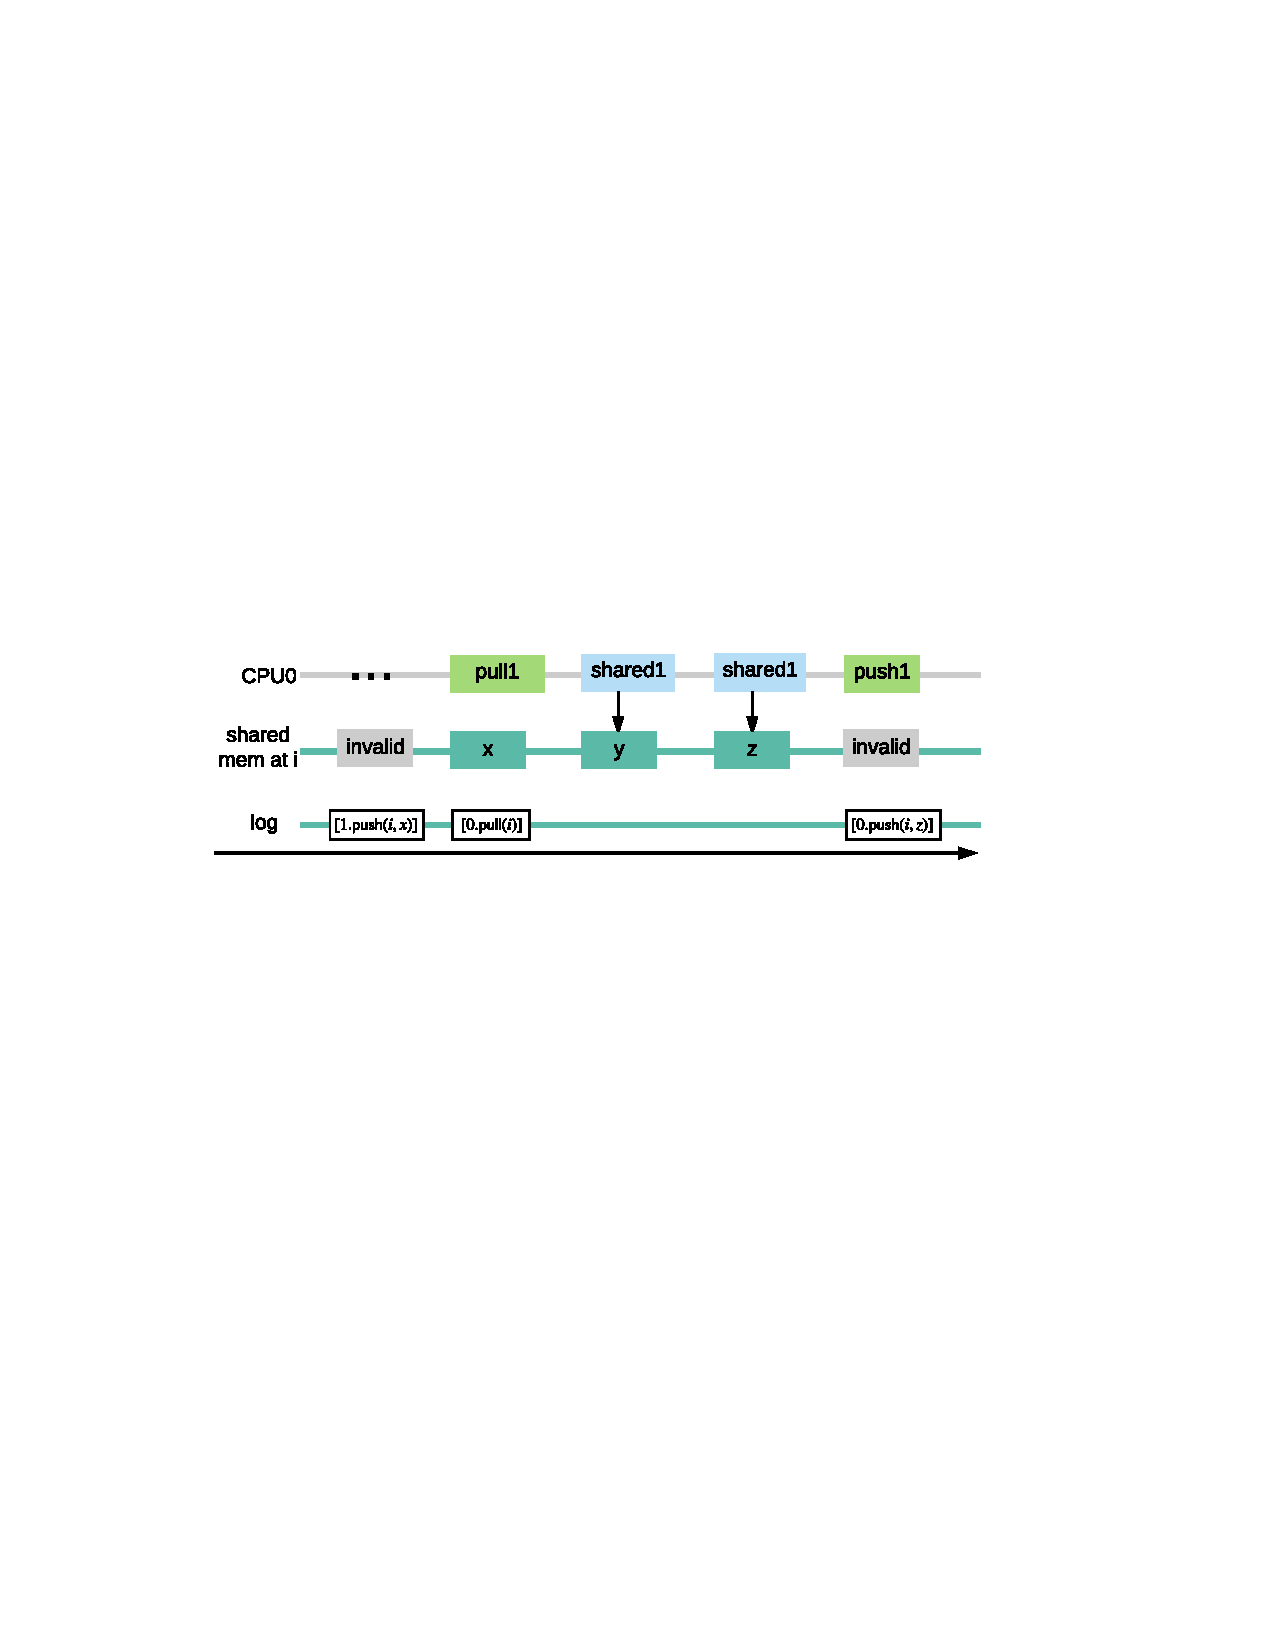
\includegraphics[scale=1]{figs/machine3}
\]
If a program tries to $\pull$ a shared memory location that is already valid,
this indicates a \emph{data race} and the machine gets \emph{stuck}.
One goal of concurrent program verification is to show
that a program is data-race free; in our setting, we accomplish 
this by showing that the program does not get stuck.

With this $\push/\pull$ model, shared memory accesses
can be treated as CPU-private executions,
whose effects to the whole machine
will be reflected by the following $\push$ operation. 

\paragraph{The transition relation $\mach{x86mc}.(\rightarrow)$}
consists of two types of transitions: 
\emph{program transitions} and \emph{hardware scheduling}, which can 
be nondeterministically interleaved.

\emph{Program transitions} can be of three types:
private transitions,
non-atomic shared transitions,
and atomic transitions.
Private transitions consist of
internal statements that only access
CPU-private memory,
and  private primitive calls.
Non-atomic shared transitions
only include 
internal statements that access shared memory.
The first two types are ``local'', 
in that they can only access CPU-private 
state and the portion of shared memory marked as valid.
In both case, the global log $l$ will not be accessed.
Atomic transitions are
shared primitives calls, 
which will access shared object
and provide the only means 
for accessing the global log and for generating events.
Both $\push$ and $\pull$ operations
are special shared primitive calls.
\ignore{
whose semantics is denoted
as the step relation $(args;s, res;s')$.
It says that starting from the state $s$ with the argument
$args$, the execution terminates with the state $s'$ and return
value $res$.}

\emph{A hardware scheduling transition} changes the
current CPU $id$ to some other $id$ 
and  can be arbitrarily interleaved with
program transitions.

This concurrent machine model $\mach{x86mc}$
reflects the nondeterministic concurrency features of 
multi-core hardware. 
One interleaving of an example program running on two CPUs
is:
\[
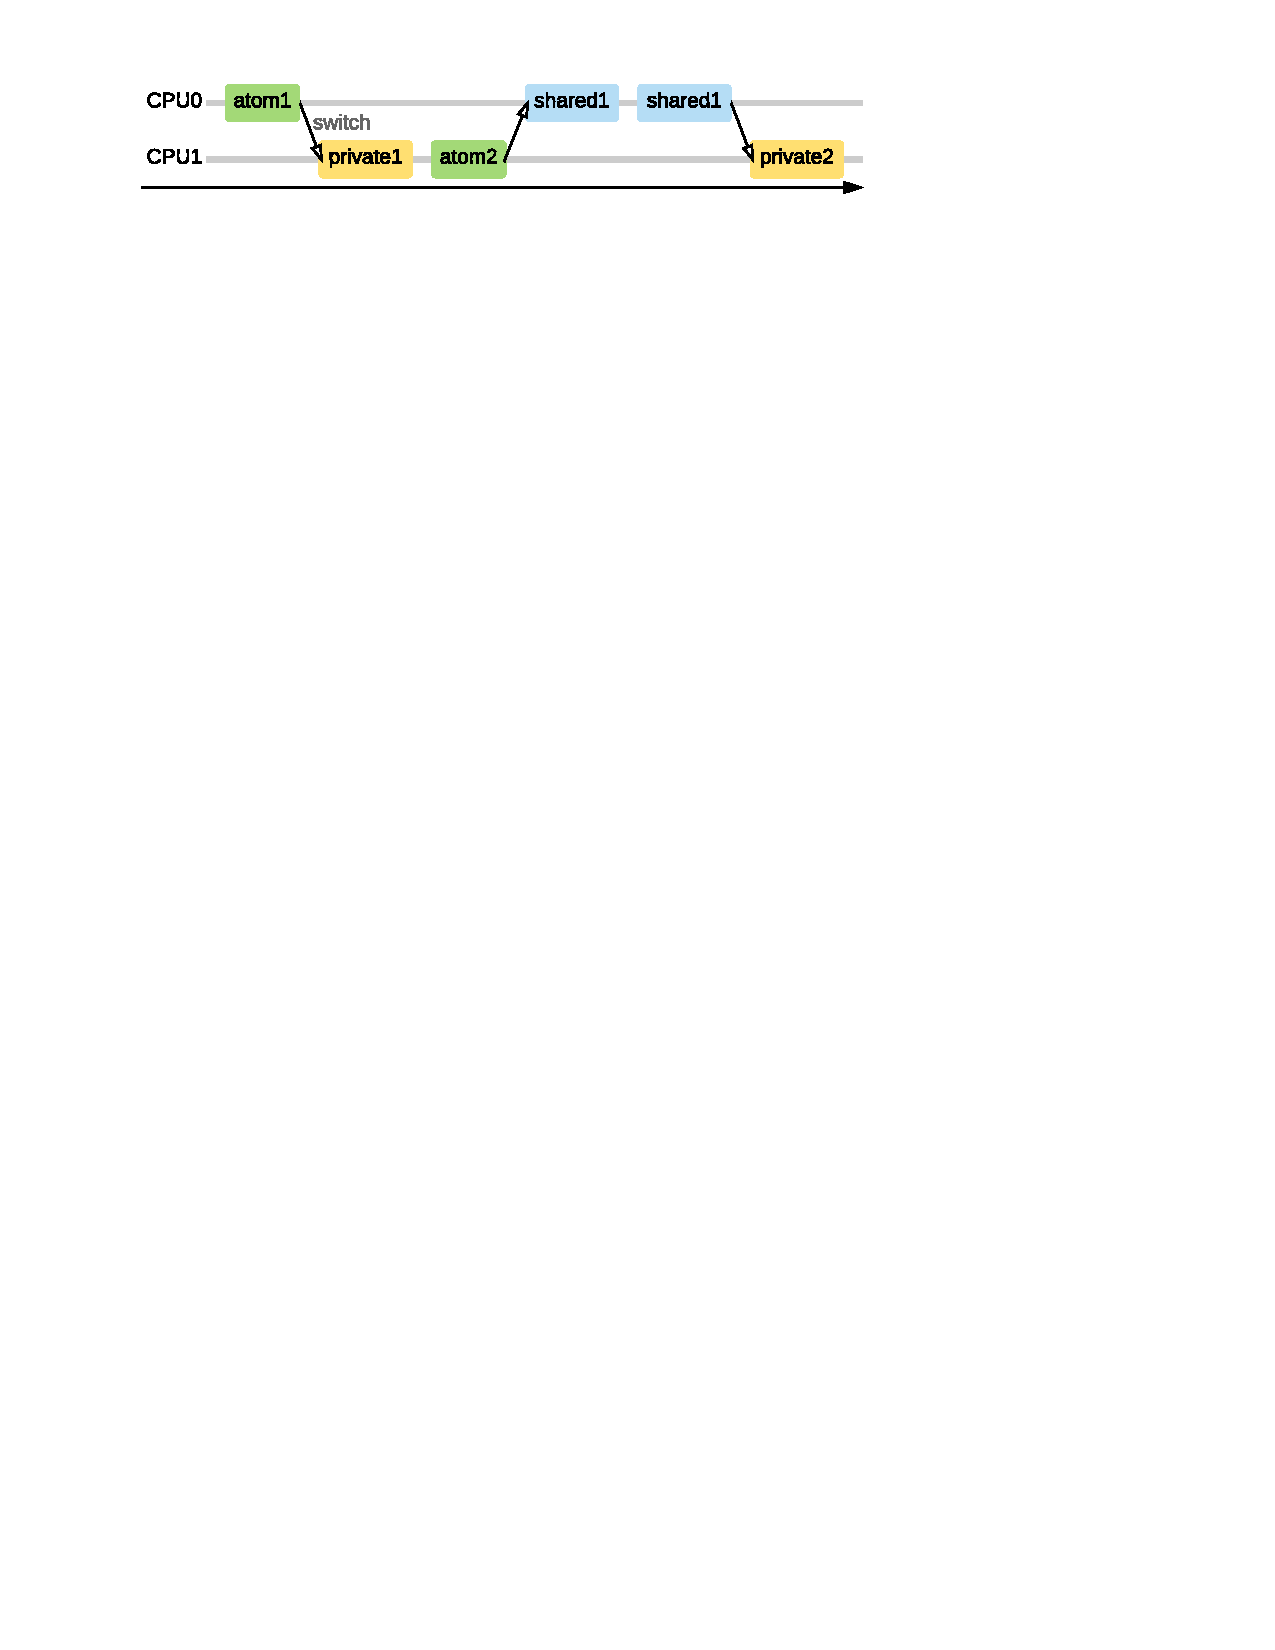
\includegraphics[scale=.93]{figs/machine1}
\]
Since only atomic transitions generate events,
this interleaving produces the logical log $[\event{0.\mathsf{atom}_1,1.\mathsf{atom}_2, 0.\pull_1,0.\push_1}]$.

\paragraph{Sequential consistency}
The \push/\pull{} memory model
assumes that the memory of the multi-core hardware
is \emph{sequentially consistent}~\cite{lamport1979make}.
Previous works~\cite{steinke2004unified,
boudol2009relaxed,owens2009better} have shown that,
for data-race free programs,
multiprocessor executions 
can be modeled as a sequence of 
shared memory access events,
which is sequentially consistent.
Therefore, by showing that the \cCTOS{}
kernel is data-race free,
we have that this sequential consistency assumption
is valid.

\subsection{Partial machine with hardware scheduler}
As a first step toward abstracting away the low-level details of
concurrent CPUs, we introduce a new partial machine ($\pmach{hs}$) configured
with a
\emph{hardware scheduler} ($\hardoracle$) that specifies a 
particular interleaving for an execution. 
This results in a deterministic machine model.
To take a program from $\mach{x86mc}$ and run it on top of $\pmach{hs}$,
we insert a  \emph{logical \intptext}
(denoted as ``$\intp$") before each assembly instruction.
Each switch point \intptext
yields to the hardware scheduler
and generates
a switch event
$c \switch hs$,
which is a \emph{local step} $\mach{hs}.\Delta$.
Then, the machine has to take
an \emph{environment step} to query the hardware scheduler
and get the CPU $id$ $c'$ to execute next.
This \emph{decision} made by $\hardoracle$ is stored in the 
log as a switch event $hs \switch c'$. 
The previous example on $\mach{x86mc}$
can be simulated by the following $\hardoracle$:\vspace{-5pt}
\[
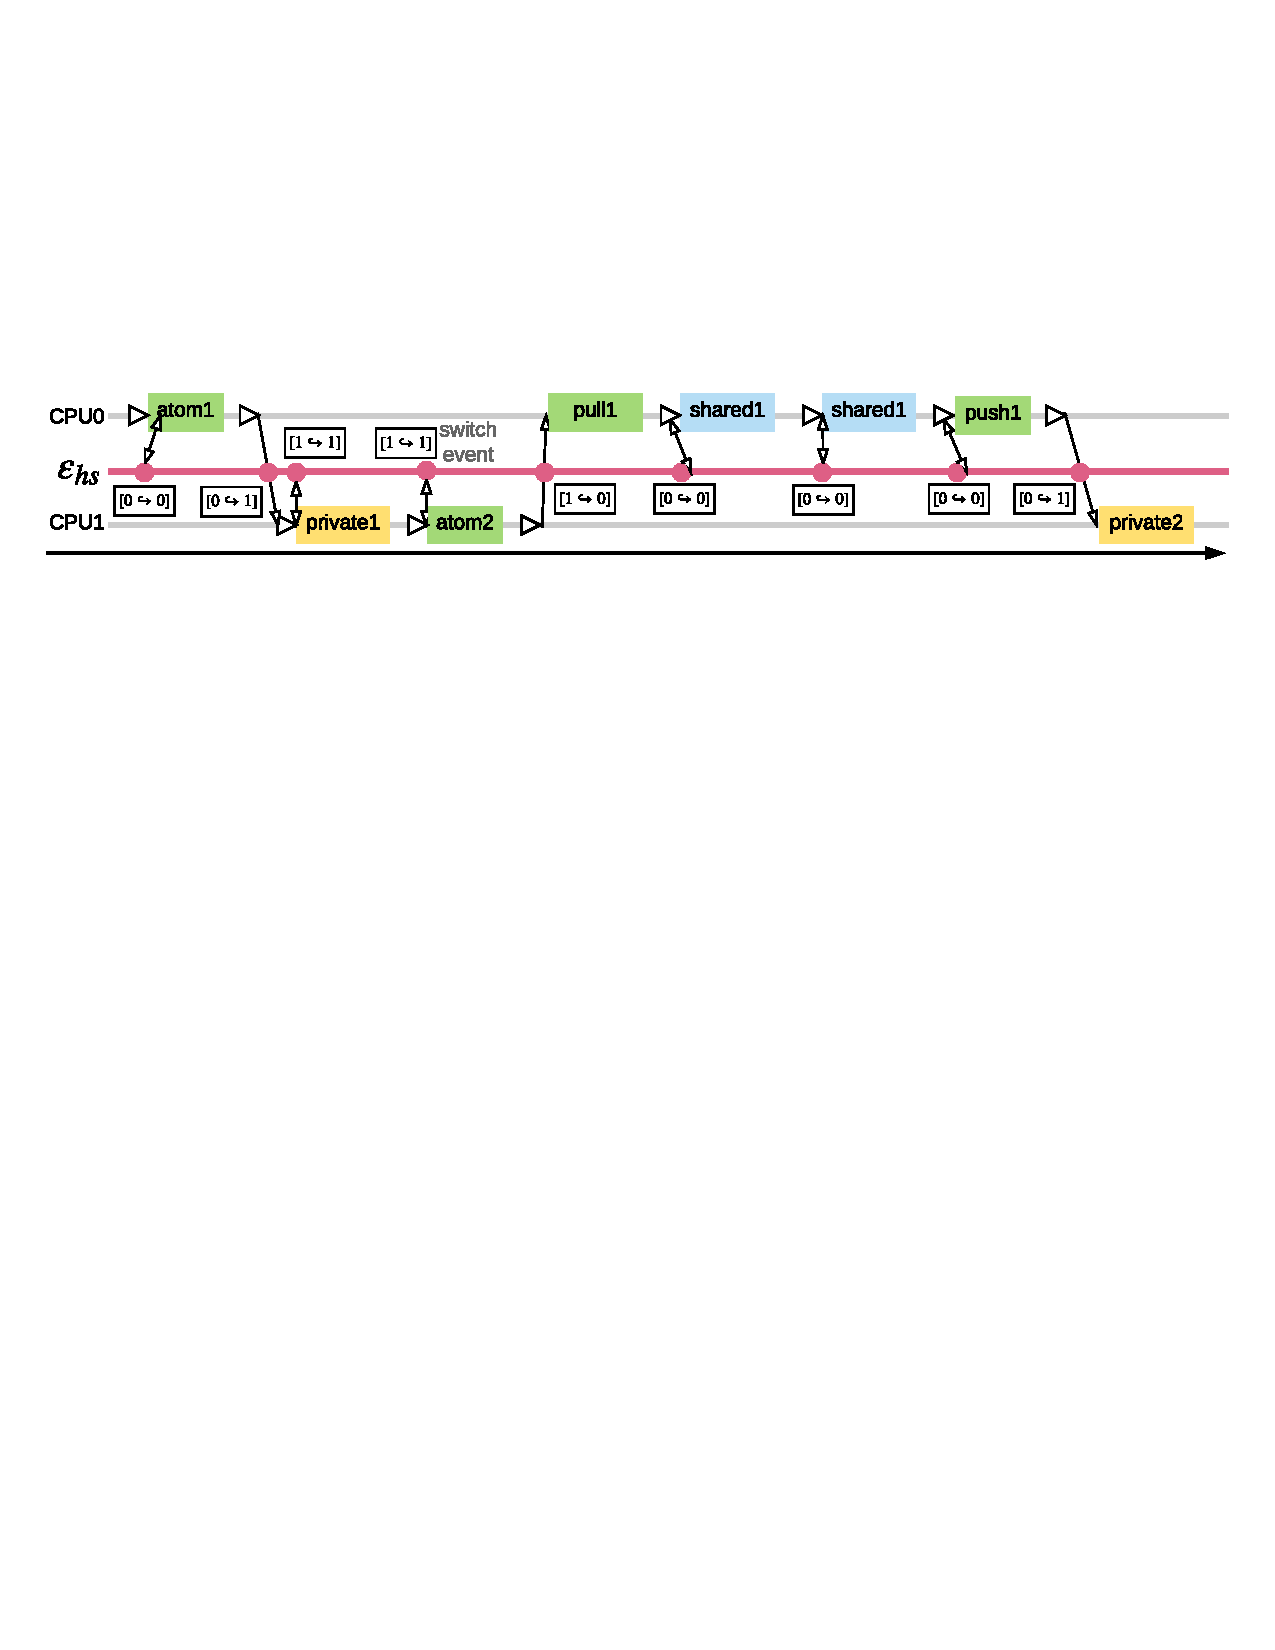
\includegraphics[scale=.75]{figs/machine2}
\]
\noindent
We write $(c \switch c')$
as an abbreviation of $(c \switch hs) \cons (hs \switch c')$.
Thus,
the log recorded by this execution is as follows:
\[
\begin{array}{l}
(0\switch 0) \cons (0.atom_1)
\cons (0\switch 1) \cons (1\switch 1)
\cons  (1\switch 1) \cons (1.atom_2)
\cons (1\switch 0) \cons (0\switch 0)
\cons ( 0\switch 1)
\end{array}
\]
\noindent
Note that this model is a special case of the partial
machine,
where the 
active set is the set of all CPUs,
and the environment is the hardware scheduler.
The \emph{rely} log invariant simply holds
on any log that the \emph{target} is $hs$:
\[\pmach{hs}.R := \{ l \in \Ev^* \ |\ \kw{target}(l) = hs \}\]
The \emph{guarantee} invariant states
two important properties:
\emph{data-race freedom}
and \emph{active consistency}.
The first property says
 that there is no
data race in the system,
\ie, there is no $\pull$ operations over $\code{valid}$
memory location and every $\push$ operation
are done following its $\pull$ operation.
The second property simply
requires that all the events
are generated by the current active CPU or the hardware scheduler.
We write $\code{well\_form}$ a predicate
over logs to state these twp properties.
Thus, the guarantee invariant is shown as below.
\[\pmach{hs}.G := \{ l \in \Ev^* \ |\ \kw{target}(l) \in \code{CPU\_set}
\land \code{well\_form}(l) \}\]
Any \emph{safe} execution of  local steps (\ie, $\pmach{hs}.\Delta$) result a log $l \in \pmach{hs}.R \cup \pmach{hs}.G$.
Thus, since the hardware scheduler only returns switch events,
the result log of any environment step still satisfies
$\pmach{hs}.R \cup \pmach{hs}.G$ regardless
of the next CPU $id$ decided by the hardware scheduler.
To ensure the correctness of this machine,
we prove that $\mach{x86mc}$ \emph{refines} this
partial machine with hardware scheduler.

\begin{lemma}[Correctness of the hardware scheduler mode]
\[\mach{x86mc} \refines \bigcup_{\oracle_{hs}}{
\pmach{hs}\langle \oracle_{hs} \rangle}
\]\proof[Proof Sketch]
For any interleaved execution on $\mach{x86mc}$, we construct
a corresponding hardware scheduler on $\pmach{hs}$.
Thus, the log of $\mach{x86mc}$
is equal to the log of $\pmach{hs}$
by removing all the switch events.
 \label{lemma:pboot}
\end{lemma}


\subsection{Partial machine with environment context}

Although $\pmach{hs}$ is deterministic
with respect to a hardware scheduler,
it still does not have much support for CPU-local reasoning.
To support modular verification, 
we should provide a \emph{partial machine}
 to reason about programs on each CPU locally by specifying
expected behaviors of the context programs on other CPUs. Thus,
we can apply the linking theorems for the partial machine
 and 
 form a global
claim about the whole system. 
To this purpose, we introduce a partial
machine model $\mach{ec}$ that can be used to reason about the
programs running on a subset of CPUs, by
parametrizing the model over the behaviors of an \emph{environment context}
(\ie, the rest of the CPUs).

The active set $A$ of the partial machine  $\pmach{ec}$
is a local subset of CPUs,
and the context contains
both other CPUs and the hardware scheduler.
At each switch point,
the machine takes an environment step
to get the next CPU $id$ to execute.
If it yields a CPU outside the active set,
it will keep taking the environment step
to get the next event generated
by the context, until yielding back to an active CPU.

\paragraph{Environment context}
of $A$ in this machine model 
is denoted as $\ectxt{\pmach{ec}^A}$.
Each environment context $\oracle_{ec}\in\ectxt{\pmach{ec}^A}$
is a \emph{response function},
which takes the current log 
and returns an event from the context CPUs
or the hardware scheduler,
which is guaranteed to satisfy some invariant.
In other words, response function simulates the observable behavior 
of the context CPUs and the potential interleaving, while the invariant states the assumptions being 
made over the context.
The execution of CPU 0 in the previous example can be simulated
with a $\oracle_{ec}$.
\ignore{$\oracle_{\overline{\set{0}}}$
(\ie, $\oracle_{\set{1}}$, since there are only two CPUs).}
\[
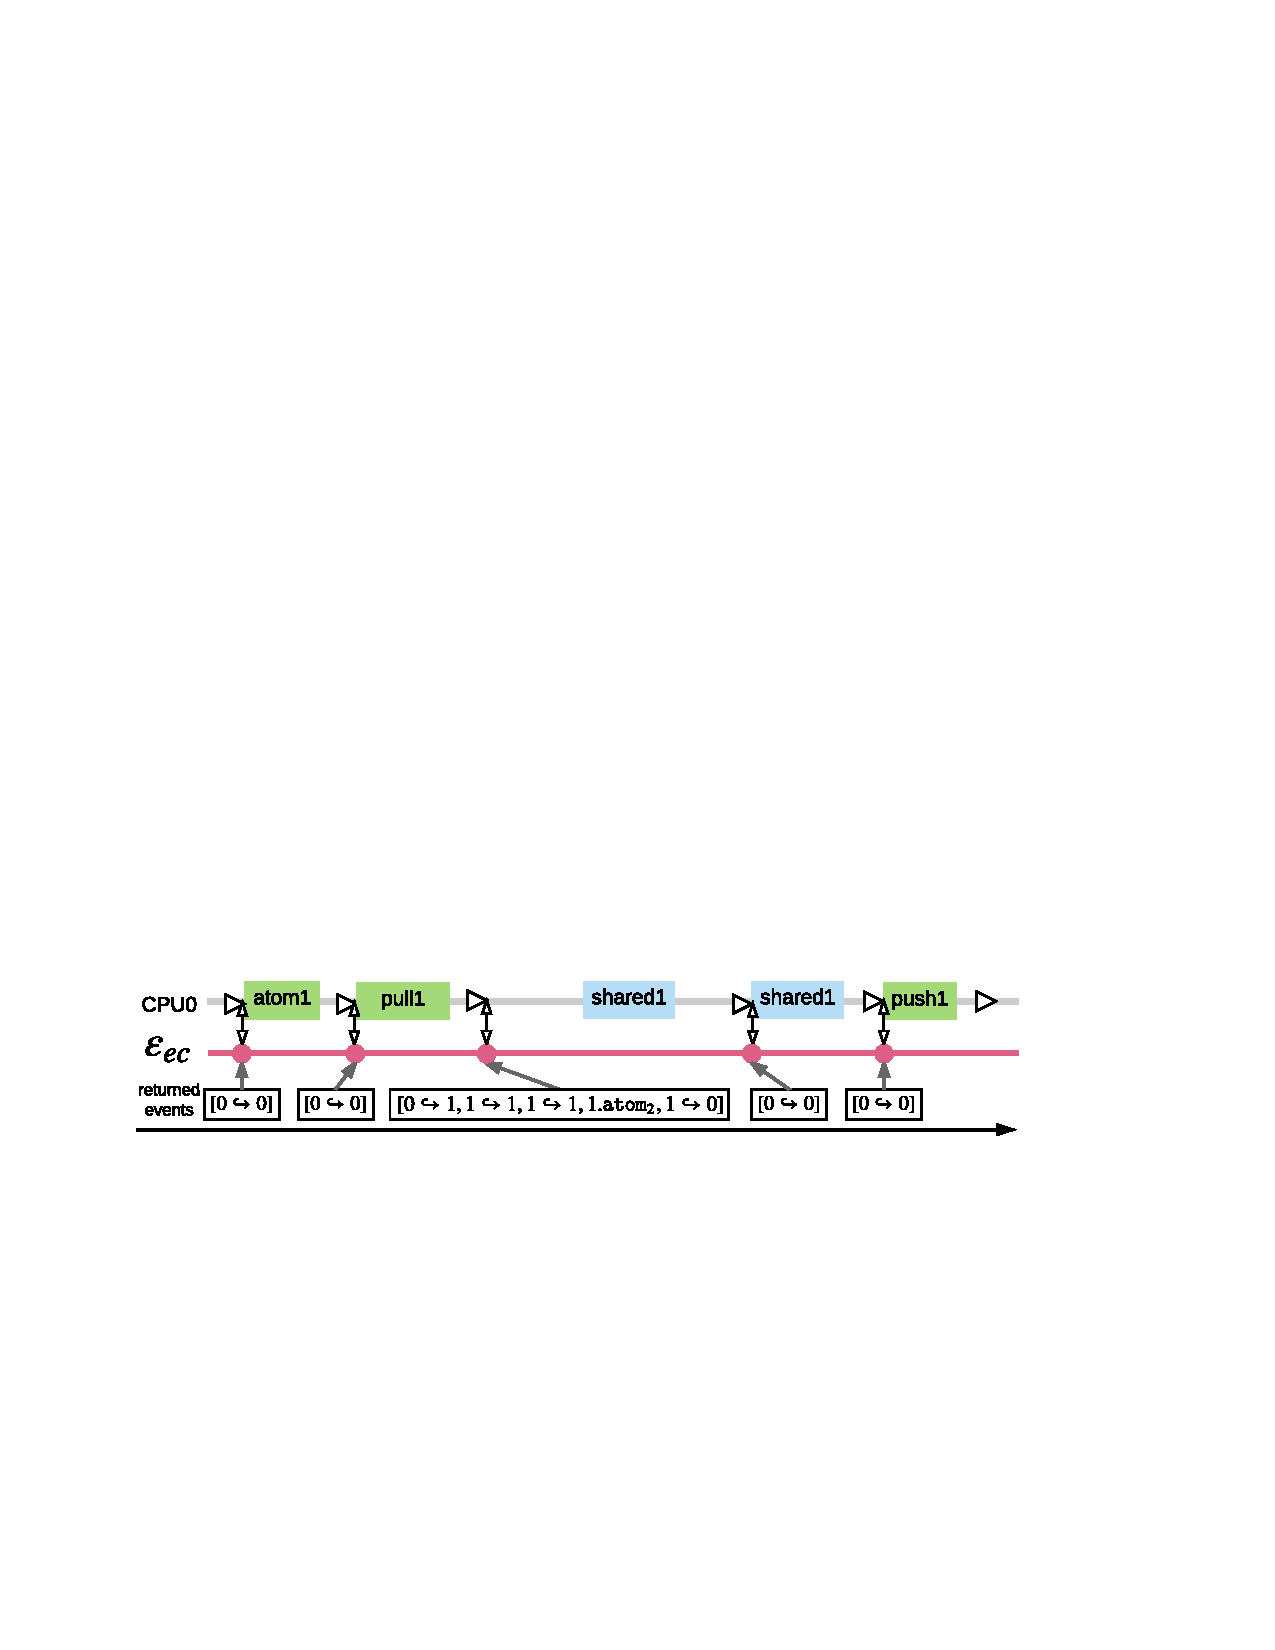
\includegraphics[scale=.9]{figs/machine4}
\]

\ignore{The environment context $\oracle_{\set{1}}$
generates the event list $[\event{0\switch 1},\event{1\switch 1},\event{1\switch 1}, \event{1.atom_2}, \event{1\switch 0}]$
at the third \intptext.}

\paragraph{Composition with environment context}
For the partial machine $\mach{ec}$,
both the rely and guarantee invariants
require the log to be well-formed.
\begin{align*}
\pmach{ec}^A.R := \{ l \in \Ev^* \ |\ \kw{target}(l) \not\in A
\land \code{well\_form}(l) \} \\
\pmach{ec}^A.G := \{ l \in \Ev^* \ |\ \kw{target}(l) \in A
\land \code{well\_form}(l) \}
\end{align*}
Therefore, for disjoint active set $A_1$ and $A_2$,
the linking operator $\Join$ is well-defined 
(\cf Definition~\ref{def:link:partial}),
and form the linked partial machine:
\[\pmach{ec}^{A_1} \Join \pmach{ec}^{A_2}
\quad \text{ if } A_1 \cap A_2 = \emptyset\]

After composing the programs on all CPUs, the context CPU set becomes
empty, and the hardware scheduler is the only context.
Since we can prove that the log generated
by any safe execution on $\mach{hs}$
is well-formed,
the environment context is  is
reduced to the \emph{hardware scheduler}
$\oracle_{hs}$, which only generates the
switch events. In other words, by
showing that this \emph{composed machine} with the entire CPU set
is refined by $\pmach{hs}$, 
all the properties proved can be propagated down to the
multicore hardware model.

\begin{lemma}[Correctness of the environment context model]
\[\pmach{hs} \refines_\id \bigJoin_{c\in\comm{CPU\_set}}
\pmach{ec}^{c}\]
\end{lemma}


\subsection{CPU-local machine}
\label{subsec:spec:seq}
If we focus on a single active CPU $i$,
the partial machine $\pmach{ec}^i$ is like a \emph{local} machine
with an environment context representing all other CPUs
and the hardware scheduler. However,
in this model there is a {\intptext} before each instruction,
so program verification still needs to handle many unnecessary 
interleavings (\eg, the ones between private operations).
In this subsection, we introduce a CPU-local
machine model (denoted as $\pmach{loc}$) for a CPU $i$, in which {\intptext}s
only appear before shared atomic operations.
The {\intptext}s before shared or private operations
are removed via two steps: \emph{shuffling} and \emph{merging}.

\paragraph{Shuffling {\intptext}s}
In $\pmach{loc}$, we introduce a \emph{log cache}~--- for
the {\intptext}s before shared and private operations,
the query results from the environment context
are stored in a temporary log cache.
The cached events are applied to the logical log
just before the next shared atomic operation.
Thus, when we perform shared or private operations,
the observations of the environment context are delayed
until the next atomic operation.
This is valid because a shared operation can only be performed
when the current local copy of shared memory is valid, meaning that 
no other context program can interfere with the operation.

\paragraph{Merging {\intptext}s} Once the {\intptext}s are shuffled properly,
we merge all the adjacent {\intptext}s together.
When we merge {\intptext}s, we also need to merge 
the switch events generated by the environment context.
For example, the change of {\intptext}s for the previous example
on CPU-local machine is as follows: 
\[
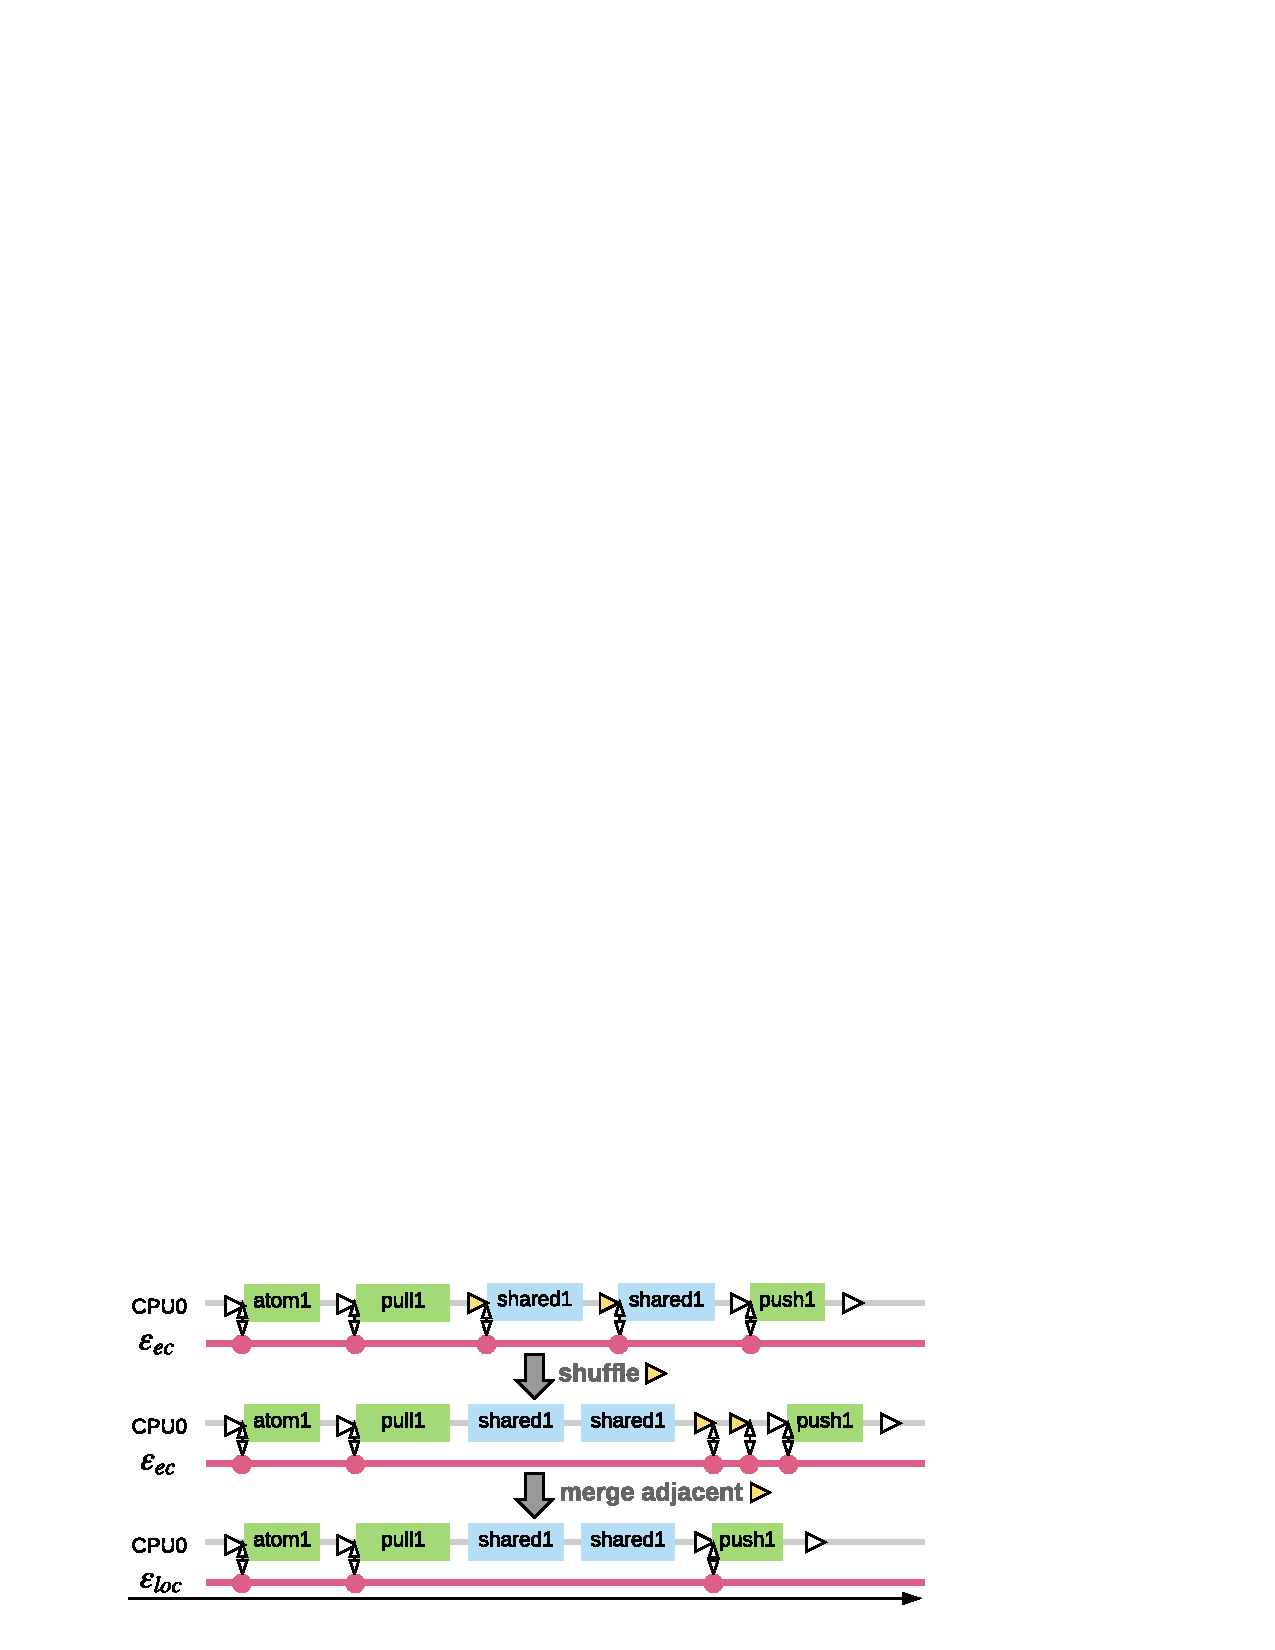
\includegraphics[scale=.9]{figs/machine5}
\]

\begin{lemma}[Correctness of CPU-local machine model]
\[\pmach{ec}^c \refines
\pmach{loc}^{c}\]

\ignore{
\[
\forall \oracle_{\overline{\set{i}}},
\exists \oracle'_{\overline{\set{i}}},
(\mach{pt},\oracle_{\overline{\set{i}}})_{\set{i}}
\machrel 
(\mach{loc},\oracle'_{\overline{\set{i}}})_{\set{i}}
\]
}
\ignore{\[
\begin{array}{l}
\forall P\ \oracle_{\overline{\set{i}}}\ \inv_{\set{i}},
\exists \oracle'_{\overline{\set{i}}},\\
\machbe{P}{\mach{pt}}{\oracle_{\overline{\set{i}}},  \inv_{\set{i}}}
\machrel 
\machbe{P}{\mach{loc}}{\oracle'_{\overline{\set{i}}}, \inv_{\set{i}}}
\end{array}
\]
\proof
Shuffling and merging {\intptext}s  are valid.
\qed}
\end{lemma}




\subsection{LAsm with concurrent layer interface}
\label{sec:con:lasm}

\ignore{
The Lemma~\ref{lemma:pboot} actually ``links'' $\PBoot$ with all
possible semantics for the hardware scheduler $hs$.}

%% Thanks to the Lemma~\ref{lemma:pboot}, the guarantees proved
%% over $\PBoot$ can be propagated down to the $\Mach_\boot$ level.

% TODO: This is wrong.
%% What's more, by the monotonicity lemma~\ref{lemma:mono},
%% we can build certified abstraction layers
%% with a single CPU $c$ on $\LAsm(L(c,\oracle))$, and compose the 
%% abstraction layers with the linking operator $\Join$.
%% In the rest of the paper, we will focus on this single-core
%% machine $\LAsm(L(c,\oracle))$.

\ignore{\paragraph{Single-core assembly machine $\LAsm(L(c,\oracle))$}}
The $\LAsm$ assembly machine model (\cf Section~\ref{sec:seq:lasm}) is
designed to ease sequential compositional reasoning. $\LAsm$ takes as
argument a sequential layer interface $L := (\abst, \primt_{\mathrm{ClightX}}, \primt_{\mathrm{LAsm}}, \invt, \mat)$
(\cf Definition~\ref{def:asm-layer}).
In the concurrent setting, we can reuse $\LAsm$ with an extended
notion of layer interface, \emph{concurrent layer interfaces}.

\begin{definition}[Multiprocessor layer interfaces]
A concurrent layer interface $L :=(\abst, \Ev, \primt_{\mathrm{ClightX}}, \primt_{\mathrm{LAsm}}, \invt, \mat)$ where 
$\Ev$ is the type for all possible events
, and, for any CPU identifier $c$ and environment 
context $\oracle$, $\primt_{\mathrm{ClightX}}(c, \oracle)$ 
and $\primt_{\mathrm{LAsm}}(c, \oracle)$ are the sets of 
available C-style and assembly-style primitives. We then write $L(c, \oracle) = ((\abst, \primt_{\mathrm{ClightX}}(c, \oracle), \primt_{\mathrm{LAsm}}(c, \oracle), \invt, \mat)$ to indicate the 
concurrent layer interface for processor $c$.
\end{definition}%
\noindent
Note $L[c]$ used in Section~\ref{sec:intro:layer}-\ref{sec:overview:concurrent}
can be viewed as a set of $L(c,\oracle)$ over any $\oracle$,
and the event type of $\oracle$ has to be consistent
with $L.\Ev$.

The $\LAsm(L(c, \oracle))$ machine state is thus defined as $\state:=(\regs, m, a, l)$,
where $\regs$ is the register set for CPU $c$,
$m$ is the memory state,
$a$ is the CPU-private abstract state,
and $l$ is the global log.
The big-step semantics of programs running on a single CPU is
almost the same with the one of LAsm,
shown in Section~\ref{sec:seq:lasm}.
Except that the machine state contains the log filed $l$,
which will not be accessed by internal steps
and non-shared primitive calls.
We write $\oracle, c \vdash L.\primt_{\mathrm{ClightX}}(i) (args,m, a, l,res,m',a',l')$ to denote
the specification of the C-style primitive
with identifier $i$,
while we write $\oracle, c \vdash L.\primt_{\mathrm{LAsm}}(j) (\regs,m, a, l,\regs',m',a',l')$ to denote
the specification of the assembly-style primitive with identifier $j$,.

Since there is a switch point $\intp$ 
in front of the shared primitive,
its semantics first query the environment context $\oracle$
with the current global log $l$
and update $l$ with the returned events generated by the environment.
We also \textbf{big-step} this query to simplify the representation,
which combines many actions.
First an switch event is
appended to the log $l$ indictating that we will interact with the
environment. Then the environment context $\oracle$ is queried
multiple times. Each time it returns an event from a CPU other than
$c$ we append that event to the log, and continue querying
$\oracle$. Finally $\oracle$ will yield back to $c$
(guaranteed by the \emph{fairness} of the hardware scheduler), and
the shared primitive call occurs.
The environment query is necessary before each shared primitive call because 
other CPUs must be given a chance to update shared state before the current 
CPU accesses it. 
\ignore{Note, however, that we do not need to worry about querying
the environment at internal statements and private primitives, since
the shared state cannot influence the behavior of these
transitions.} In the following, we will abuse notation and write
$l \cons \oracle(l)$ to mean the entire process of extending $l$ with
multiple events from other CPUs.
\ignore{which means that, starting from the log $l$, $\oracle(l)$ keeps
querying and appending events until the destination
is the current CPU $c$.}

In most cases, the execution of a primitive depends on what events have
been triggered at the switch point. 
For example, the $\pull$ primitive returns the
current state of the shared memory, which depends on what shared
memory updates from other CPUs are recorded in the global log.
To write the primitive specifications, we introduce an idiom of a
\textbf{replay function} $\replay$, which takes a
log as an argument, and interprets it to calculate the ``current
state'' of the system after those events have happened. The
result of the replay function can be an arbitrary type, corresponding
to what kind of information is needed about the shared operations.

For example, the replay function $\replay_{\comm{get\_shared}}$
reconstructs the shared memory state from the given log.
It first retrieves the last shared memory
update to location $b$ from the log $l$. If the last update is
$c.\pull(b)$, it returns $(\any, \comm{invalid})$, where $\any$ denotes
any possible value. The shared memory state returned in this case
does not matter since the $\pull$ operation invalidates the corresponding
memory block. On the other hand, if the last update
is $c.\push(b,\comm{bl})$ for some byte list $\bytelist$,
it returns $(\comm{bl}, \comm{valid})$. 
If there is no $\push$ or $\pull$ event in the log, it returns
$(\any, \comm{valid})$. We write ``$f\set{b:v}$"
to denote an update to the partial function $f$ at field $b$ 
with value $v$.
The rules for $\pull$ and $\push$ are defined as below:
\begin{small}
\begin{mathpar}
\inferrule{
   l_0 = l \cons \oracle(l) \\ 
  (\bytelist,  \comm{valid}) = \replay_{\comm{get\_shared}}(l_0, b) \\
  	m' = m \set{b: \bytelist} \\
  	a' = a \set{\perm{b}: \comm{valid}}  \\	
   l' = l_0 \cons c.\pull(b) \\ 
}{
 \oracle, c \vdash  \spec_{\pull}([b],\regs, m, a, l,\any, \regs,  m', a', l')
} 
\and
\inferrule{
  m(b) = \bytelist \\
  a.\perm{b} =  \comm{valid} \\
  a' = a \set{\perm{b}: \comm{invalid}} \\
  l' = l \cons  \oracle(l) \cons c.\push(b,\bytelist)   
}{
 \oracle, c \vdash  \spec_{\push}([b], \regs, m, a, l,\any, \regs, m, a', l')
}
\end{mathpar}
\vspace{-5pt}
\end{small}%

The $\pull$ operation requires the shared memory to be marked as valid
(after replaying the log). It first queries the environment context to update
the log, and then it updates the shared memory at location $b$ with the byte
list $\bytelist$ reconstructed from the log. This specification
captures the fact that the shared memory contents may be
modified by the environment context before the execution of
primitives. 
The $\push$ operation first gets the updated log from the environment context,
and then appends an event $c.\push(b,\bytelist)$ to the end of the log.
The operation is only defined when the permission bit is valid (\ie, the previous push
has already been pulled), and it invalidates the permission upon $\push$.

Let $L_\boot$ be the multiprocessor layer interface with the same abstract state, shared events, and primitives as in $\pmach{loc}$.
\ignore{
In general, $\LAsm(L(c, \oracle))$ is, however, not a partial machine.  For the
layer $L_0$ corresponding to primitives of $\mach{\boot}$, we have
constructed a partial machine $\XAsm(c)$ for a given core $c$ such
that:

\begin{lemma}
There exists a function $f$ such that, for any environment context $\oracle$: \[ \PBoot(\oracle) \refines \bigJoin_{c} \XAsm(c)(f(c, \oracle)) \]
\end{lemma}

\begin{lemma}
For any core $c$ and for any environment context $\oracle$: \[ \XAsm(c)(\oracle) \refines \LAsm(L_0(c, f(\oracle))) \]
\end{lemma}
\tahina{TODO: define $\XAsm$ and explain the proof}
}
Then,\ignore{For the layer $L_\boot$ corresponding to primitives of $\Mach_\boot$, } we
have proven that $\LAsm(L_\boot(c, \oracle))$ can be represented as a
partial machine, so that we can state and prove the following:
 \begin{lemma}
$ \forall \oracle.\ \pmach{loc}^c\langle \oracle \rangle \refines \LAsm(L_\boot(c, \oracle)) $
 \end{lemma}

\begin{figure}[t]\centering
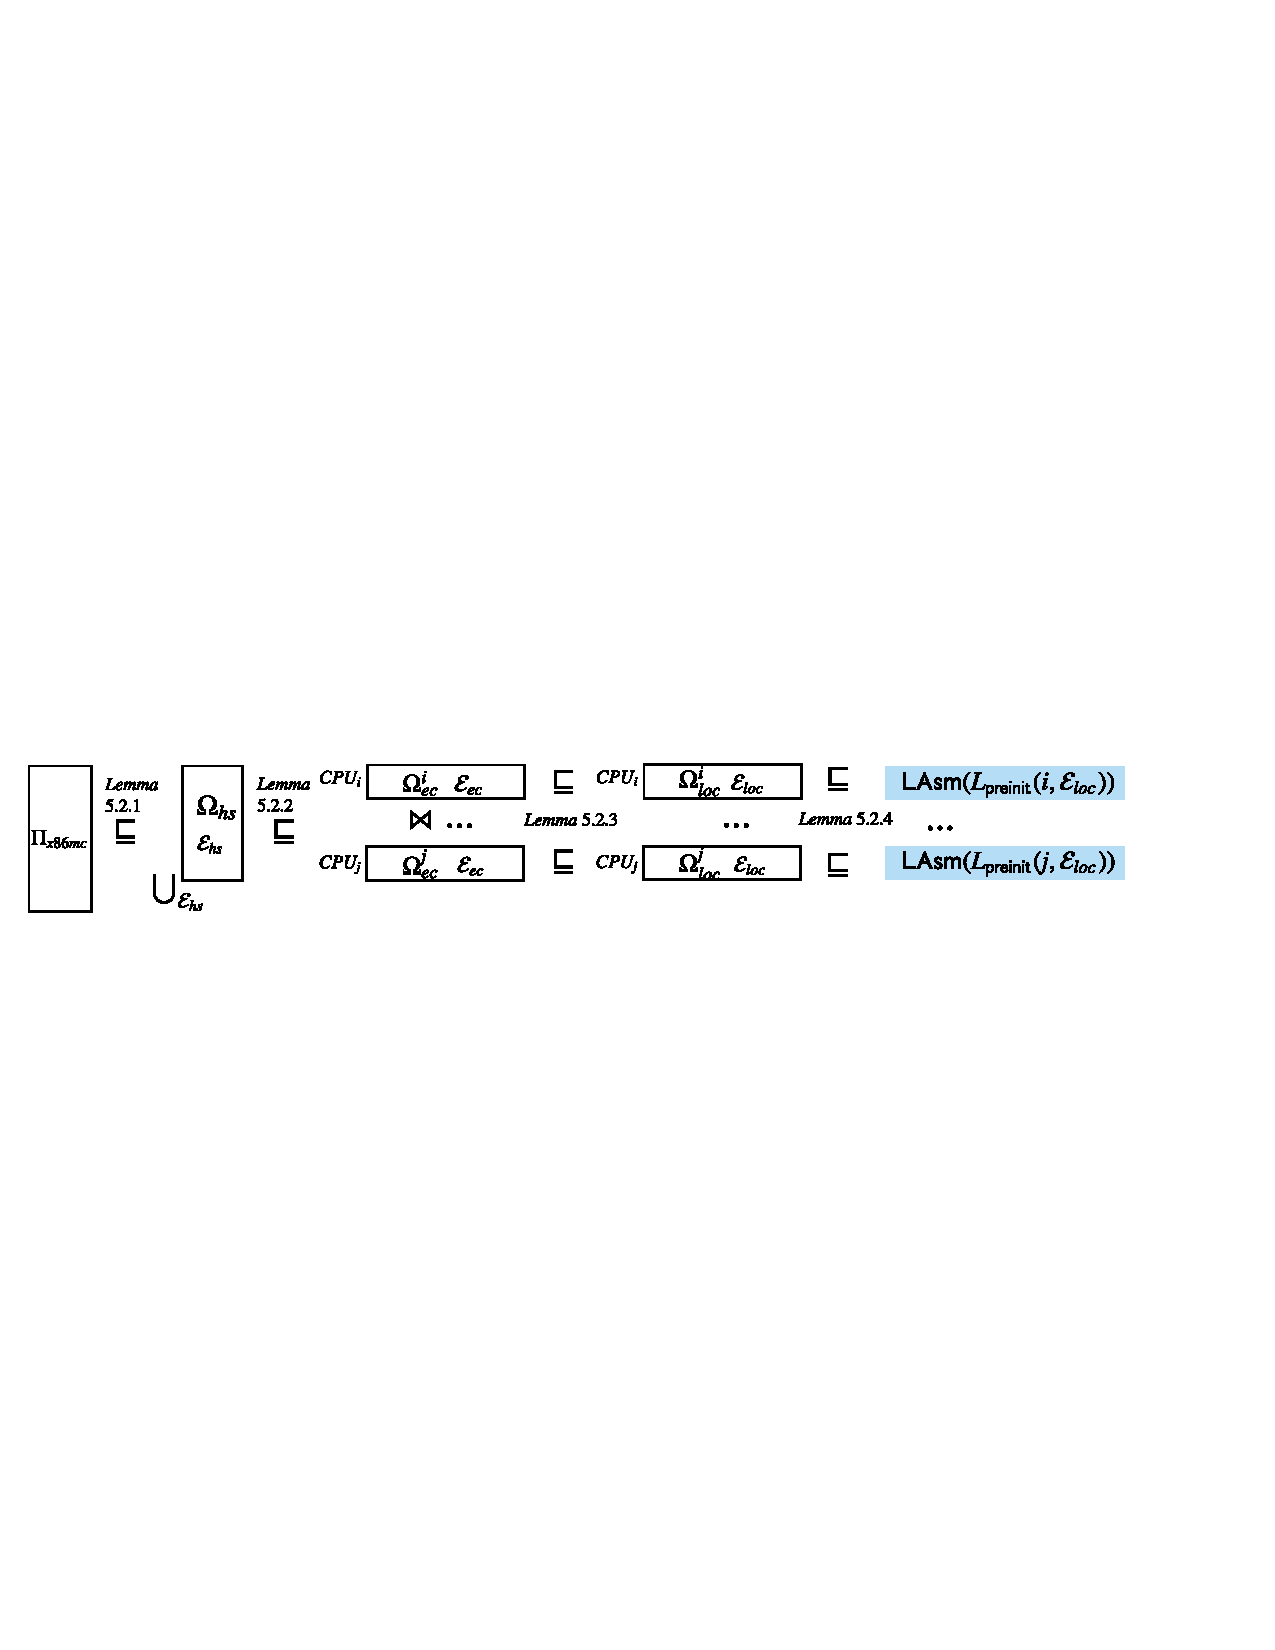
\includegraphics[scale=0.8]{figs/machine_chain}
\caption{The contextual refinement chain from multicore hardware model
$\mach{x86mc}$ to the LAsm machine
with single-core concurrent layer.}
\label{fig:spec:chain}
\hrulefill
\end{figure}

Finally, we obtain the refinement relation from the multicore
hardware model
to the single CPU LAsm machine model by composing
all of the refinement relations together (\cf Figure~\ref{fig:spec:chain}).
We introduce and verify the {\cCTOS} kernel on top of the
single CPU LAsm machine,
where the semantics of internal statements
and private primitives can be viewed as sequential,
and one only needs to consider concurrency
and interleaving at switch points (\ie, just before 
shared primitive calls).
The refinement proof guarantees that the proved properties can be
propagated down to the multicore hardware model $\mach{x86mc}$.


     % Concurrent Abstraction Layers (1.5 pages)
%%\sectskip
\vspace{-5pt}
\section{Layers with Environment Context}
\label{sec:machine}


\begin{figure}
\begin{center}
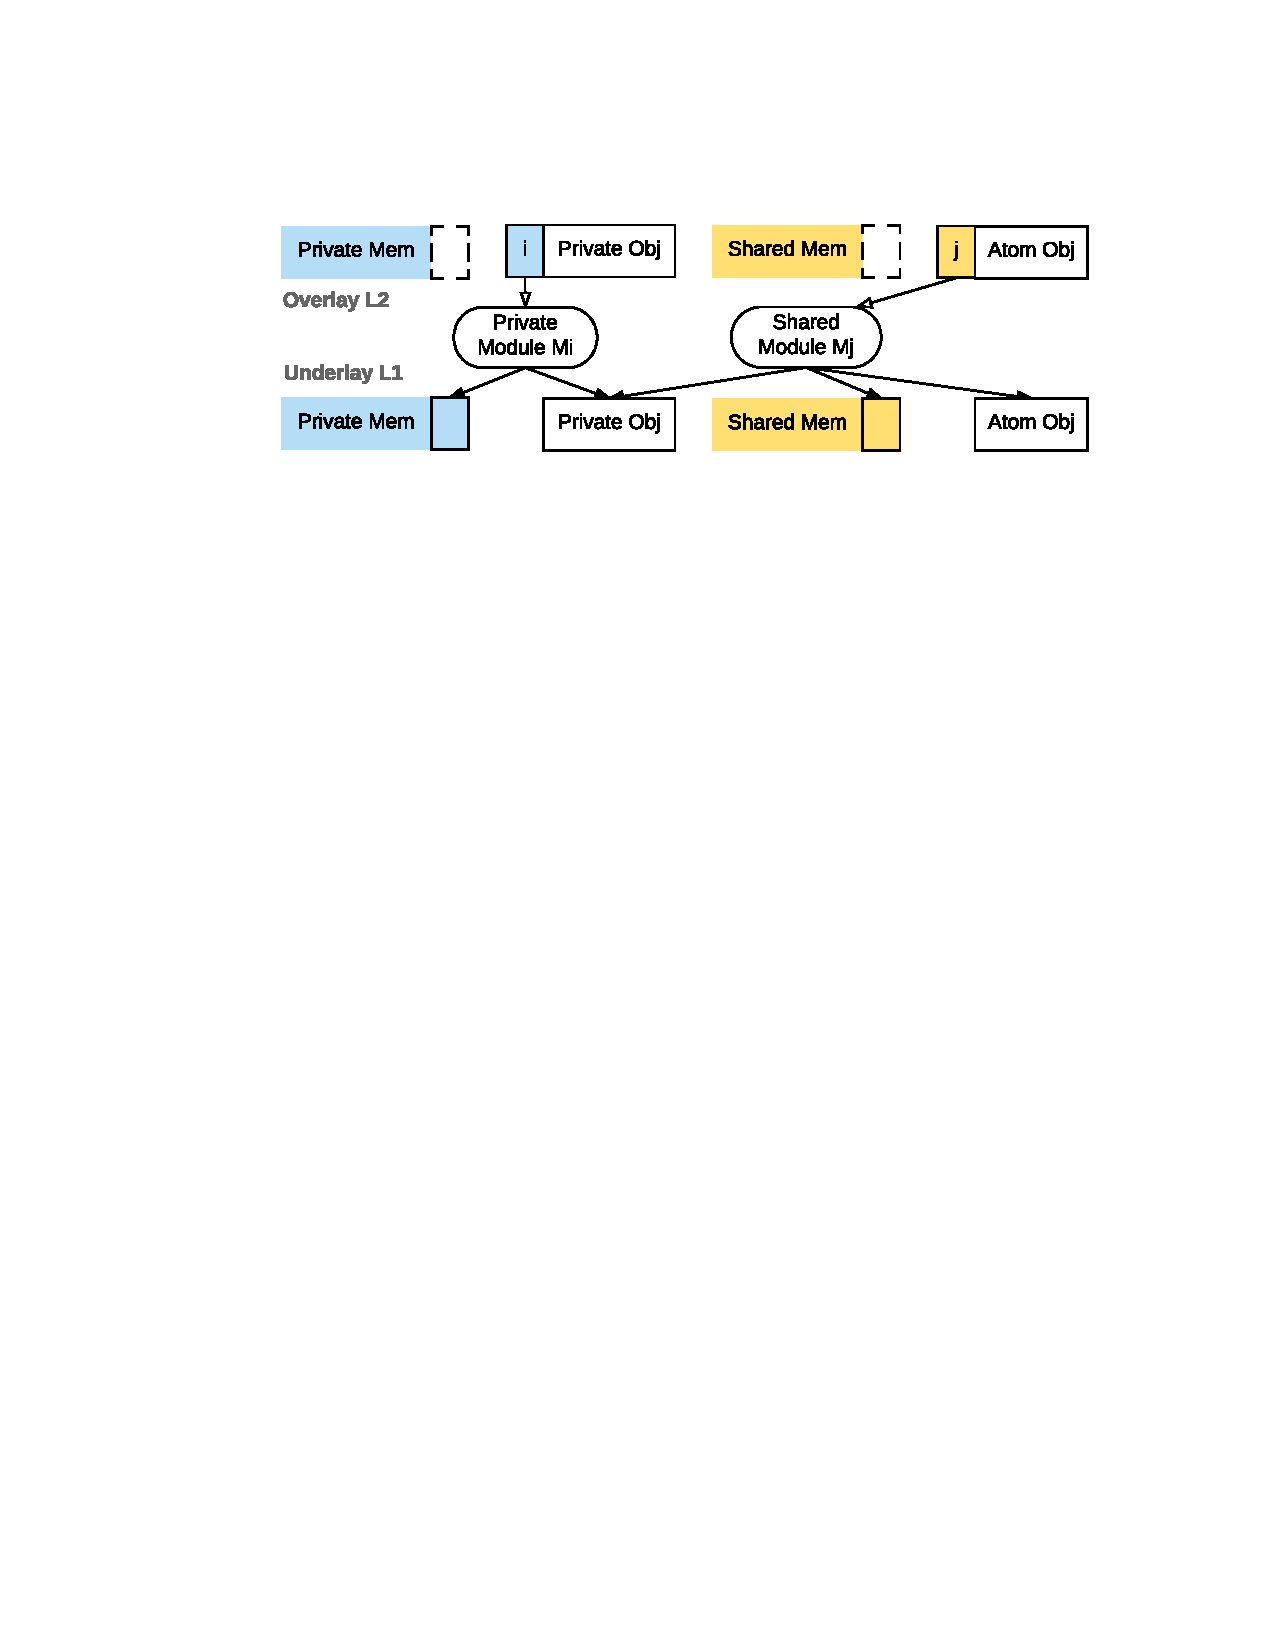
\includegraphics[scale=0.55]{figs/build_object}
\vspace*{-8pt}	
\end{center}
\caption{Defining concurrent abstraction layers.}
\label{fig:spec:object}
\vspace*{-10pt}
\end{figure}


In this section, we explain the general layer design principles and present
how we use environment context to convert a concurrent layer into 
 CPU-local layers.
\ignore{that is suitable for reasoning about concurrent code in a CPU-local way.}

\vspace*{-3pt}
\paragraph{Multicore hardware} allows
all the CPUs to access the same piece of memory
simultaneously.
In {\CTOS}, we \emph{logically} distinguish the \emph{private memory} 
(\ie, private to a CPU or a thread) from the \emph{shared memory} 
(\ie, can be accessed by multiple CPUs or threads). 
The private memory does not
need to be synchronized, whereas non-atomic
shared memory accesses need to be protected by some synchronization mechanisms
(\eg, locks), which are normally implemented using atomic hardware instructions
(\eg, fetch-and-add). With proper protection,
each shared memory operation can be viewed as if it were atomic.

\vspace*{-3pt}
\paragraph{Atomic object}
\ignore{In {\CTOS}, we refine each piece of shared data with well synchronized operations
into an \emph{atomic object}. An atomic object}

is an abstraction of well-synchronized shared memory, combined
with operations that can be performed over that shared memory.
It consists of a set of
primitives, an initial state, and a \emph{logical log} containing the entire
history of the operations that were performed on the object during
an execution. Every primitive invocation
records a \emph{single} corresponding event in the log. 
We require that these events contain enough information to derive the
current state of an atomic object by replaying the entire log starting 
from the object's initial state.
\ignore{ 
Note that every atomic primitive at the overlay always generates
exactly one event (this is how we make sure that it is really atomic),
while the actual implementation may trigger multiple events (by
calling multiple atomic primitives at underlay). The events are are
shuffled and merged during the contextual refinement, which we explain
in more detail in the subsequent subsections.
}

\vspace*{-3pt}
\paragraph{Concurrent layer interface}
$L$ is a collection of both \emph{private objects} and \emph{atomic objects},
along with some invariants imposed on these objects.
The verification of a concurrent kernel 
requires repeatedly 
building certified abstraction layers $(L_1, M, L_2)$.
The overlay interface $L_2$ is a
new and more abstract interface
built upon the underlay interface $L_1$ using module $M$
 (\cf Fig.~\ref{fig:spec:object}).
\emph{Private objects} are built from private modules with 
only private memory accesses
using techniques similar to those presented by Gu {\it et al} \cite{dscal15}. 
\emph{Atomic objects} are built from the 
existing atomic objects, private objects,
and modules with non-atomic shared memory accesses.

\ignore{
The framework requires the defined invariants to hold at any point in
the program execution. Invariant proofs are found to be particularly
challenging even in the sequential setting, where in many cases,
some invariants are temporarily violated and re-established later \cite{klein2009sel4}.
In {\CTOS}, thanks to our layered approach, we can impose different invariants
at different abstraction layers. The primitives at underlay can be hidden if they
are no longer needed at overlay, such that stronger invariants can be introduced
at some overlay with atomic primitives, which could otherwise be violated by the
lower-level primitives at underlays.
}

\ignore{
\paragraph{Verification task}
The major task to verify a concurrent kernel
is to show that kernel modules with shared memory accesses
have atomic interfaces.
In other words, the verification of a concurrent kernel
is a procedure to 
build new atomic objects based on the 
existing atomic objects, private object,
and non-atomic shared data
(\cf Fig.~\ref{fig:spec:object}).}
 
\vspace*{-3pt}
\paragraph{Verification task}
It is difficult to build certified abstraction layers
directly on
a multicore, nondeterministic hardware model. To build an atomic object,
one must reason about all of the unnecessary interleavings (\eg, the interleavings
between private operations), and prove that every access to shared memory is
well synchronized. Furthermore, it is not clear how we can reason about threads
running on each core locally and combine the proofs to obtain a global claim about the whole system.

In the remainder of this section, we first present our x86 multicore machine model
($\mach{x86mc}$), and then show how we gradually refine this low-level model into a
more abstract machine model ($\mach{loc}$) that is suitable
for reasoning about concurrent code in a CPU-local fashion.

\begin{figure*}
\begin{center}
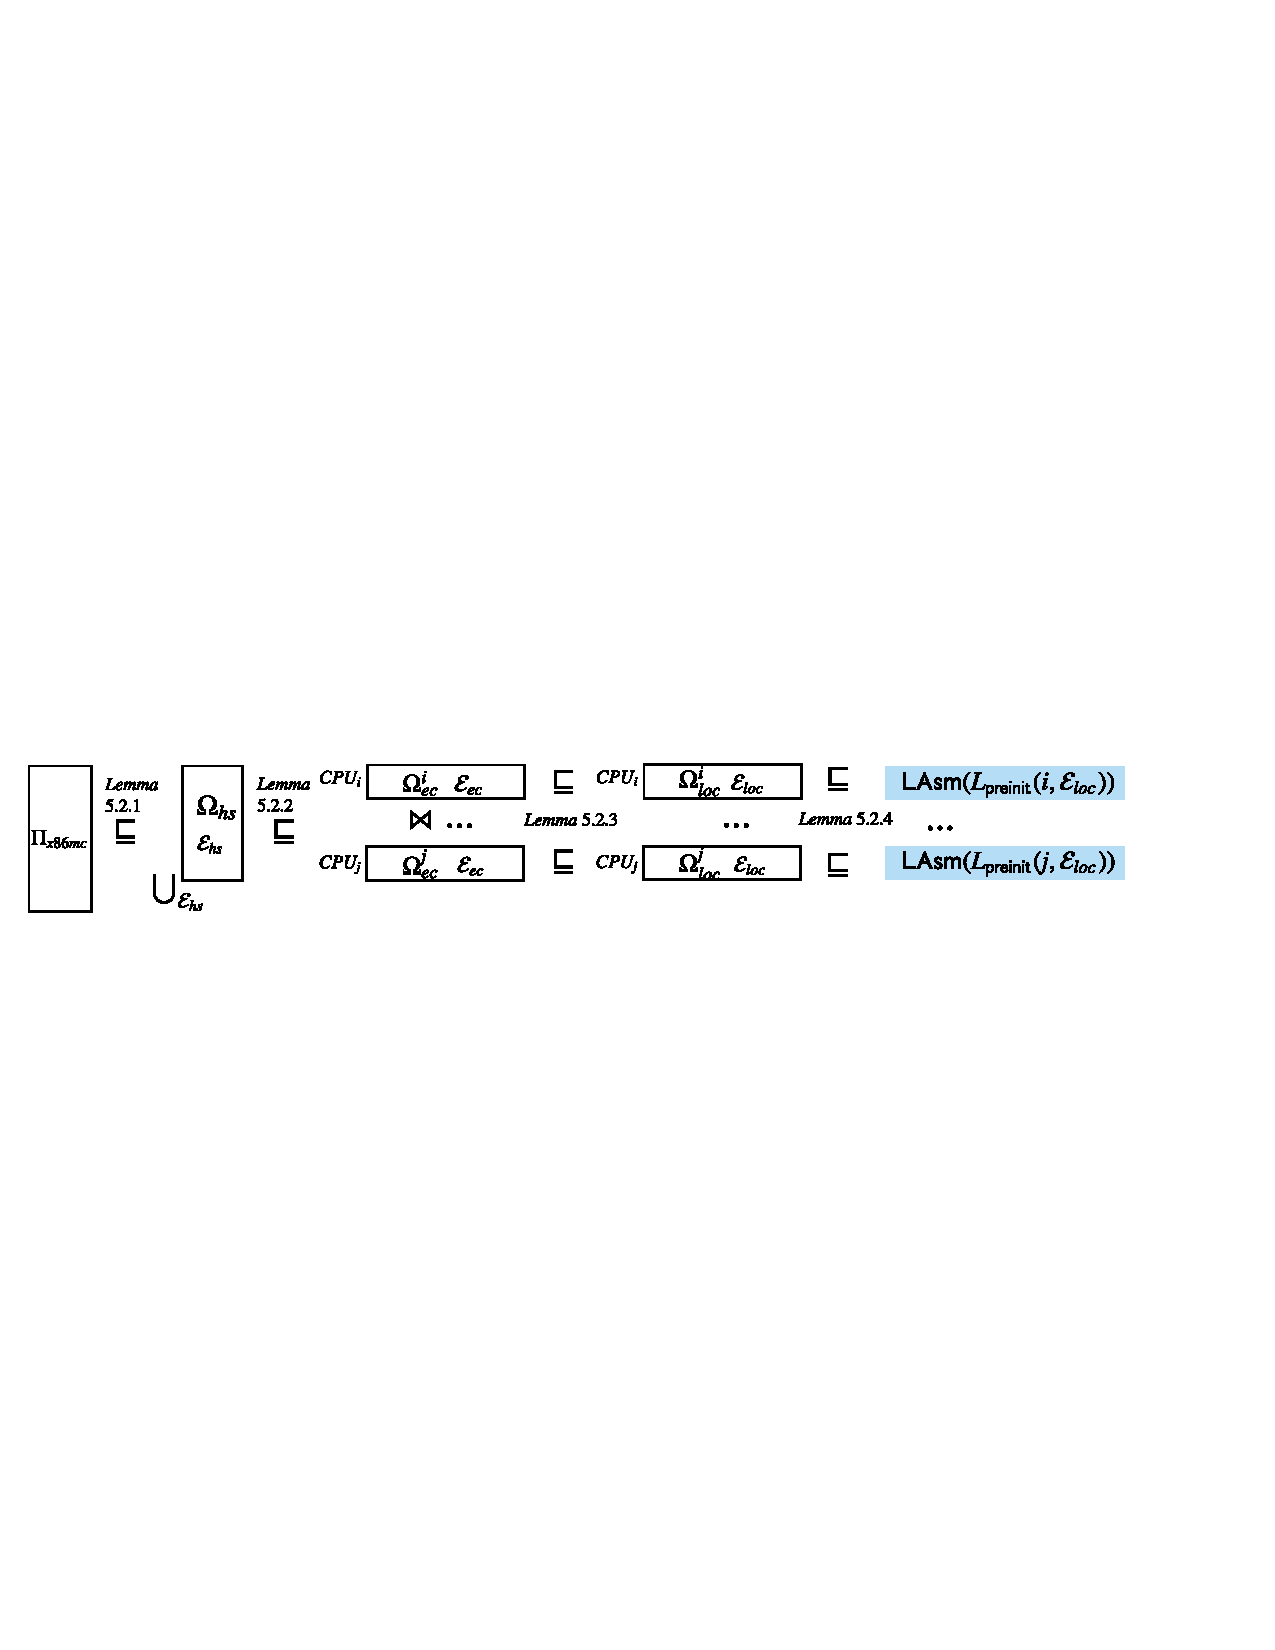
\includegraphics[scale=0.8]{figs/machine_chain}
\vspace*{-8pt}	
\end{center}
\caption{The contextual refinement chain from multicore hardware model
$\mach{x86mc}$ to CPU-local model $\mach{loc}$.}
\label{fig:spec:chain}
\vspace*{-10pt}
\end{figure*}

\vspace*{-2pt}
\subsection{Multicore hardware model}
Our fine-grained multicore hardware model ($\mach{x86mc}$) allows arbitrary
interleavings at the level of \emph{assembly instructions}.
At each step, the hardware \emph{randomly} chooses one CPU 
and executes the next assembly instruction on that CPU.
Each assembly instruction is classified as \emph{atomic}, \emph{shared},
or \emph{private}, based on if it involves an atomic object call,
a  non-atomic shared memory access, or only a private 
object/memory access.
One interleaving of an example program running on two CPUs
is:\vspace{-5pt}
\[
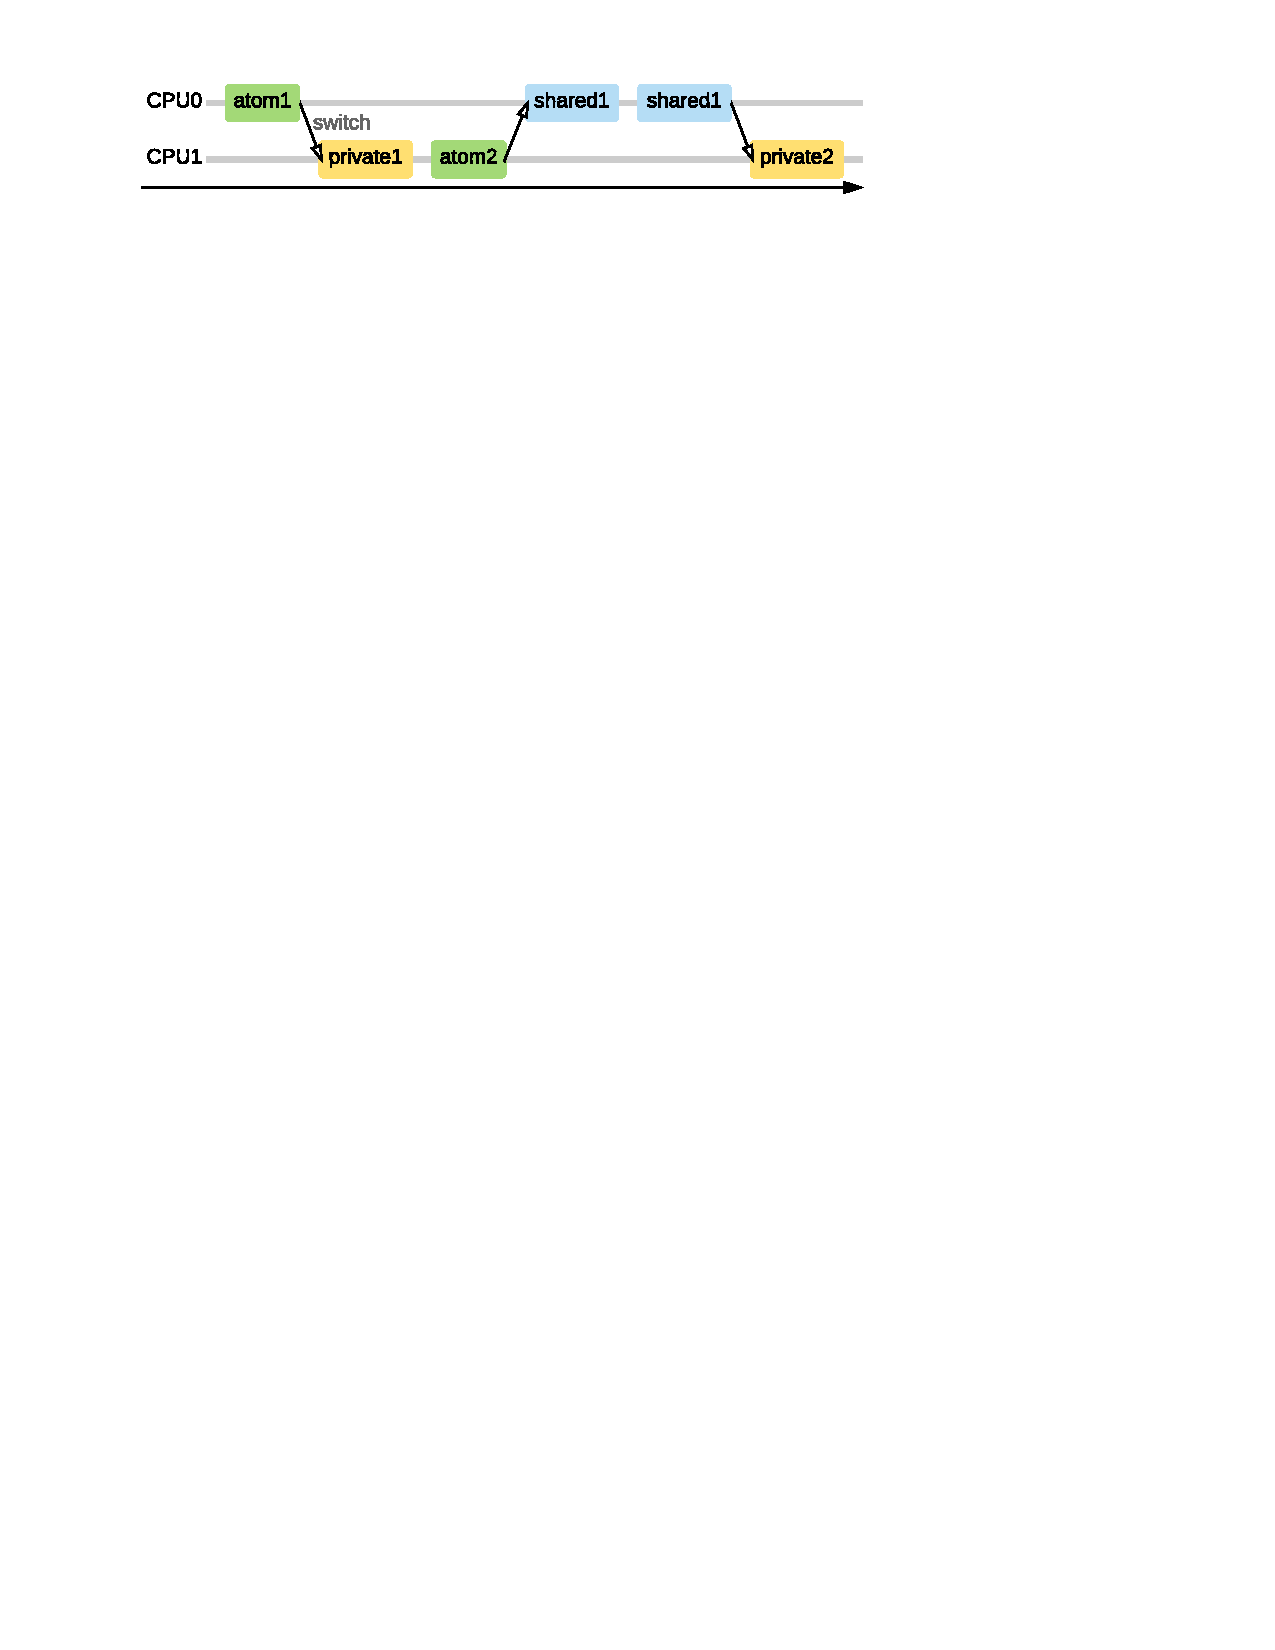
\includegraphics[scale=.65]{figs/machine1}
\vspace{-5pt}
\]
Since only atomic operations generate events,
this interleaving produces the logical log $[\event{0.atom_1,1.atom_2}]$.
\ignore{
Note that, while we mentioned above that each atomic object has its own
logical log, our model will actually maintain only a single log throughout an
execution. To obtain a per-object log, one can simply ignore all events in the
log that do not pertain to the desired atomic object.}

\ignore{
\paragraph{Memory model}
\ignore{
\ronghui{Maybe we do not need to talk about Compcert memory model?}
Because we use CompcertX~\cite{dscal15} along with
its formalization of the semantics of C and assembly,
our notion of memory is based on the CompCert memory model~\cite{leroy08}.
CompCert employs a unified model
to encode different views of memory.
The memory is split into a number of disjoint blocks and
a pointer is represented by a pair $(b, o)$, where
$b$ is a block identifier and
$o$ is an offset within block $b$.
Each offset within a block is associated with a permission
specifying the memory operations that can be performed at that location.
A program which attempts to perform a prohibited operation will \emph{get stuck}.
}

We \emph{logically} divide the machine memory into three parts:
\emph{atomic object}, \emph{shared memory},
and \emph{private memory}.
An \textbf{atomic object}
is accessed only through atomic operations
(\eg, compare-and-swap) provided by the hardware. Since these atomic operations
(denoted as \code{atom\_op})
are expensive, they are only used to implement the synchronization mechanisms
(\eg, locks). In our hardware model, each atomic operation generates 
\emph{exactly one event} that is recorded in a 
list of atomic events called a \emph{logical log}.
As shown in the ticket lock example \ronghui{reference?},
both \emph{ticket} and \emph{now} fields belong to the atomic object
and their operations generate the events $\event{inc\_ticket}$
and $\event{get\_now}$. Each method on the atomic object is considered
as atomic (as specified in the hardware manual) and its interface
is represented as a single
event. The values of an atomic object can be reconstructed from its logical log. 
\newman{I assume the events, log, and replay functions will be defined somewhere
in the Overview section?}

Operations to access shared memory and private memory
are denoted as \code{shared\_op} and \code{private\_op}, respectively.
Distinguishing between these makes it easier to reason about CPU-local 
execution.


\paragraph{Building atomic objects}
Shared memory accesses are not atomic. 
To ensure safety of the kernel,
shared memory has to be protected by synchronization
methods implemented using atomic objects.
The main task when verifying shared modules is to show that
each operation over shared memory can be viewed as if it were
atomic, provided the access is well synchronized by the atomic objects.
Therefore, concurrent kernel verification can be viewed as a procedure
to build concurrent objects with atomic interfaces (\cf Sec.~\ref{subsec:layer_def}).

\paragraph{Interleaving semantics}
}

\vspace*{-2pt}
\subsection{Machine model with hardware scheduler}
As a first step toward abstracting away the low-level details of
concurrent CPUs, we introduce a new machine model ($\mach{hs}$) configured
with a
\emph{hardware scheduler} ($\hardoracle$) that specifies a 
particular interleaving for an execution. 
This results in a deterministic machine model.
To take a program from $\mach{x86mc}$ and run it on top of $\mach{hs}$,
we insert a  \emph{logical \intptext}
(denoted as ``$\intp$") before each assembly instruction.
At each \intptext, the machine first queries the hardware scheduler
and gets the CPU ID to execute next.
All the \emph{switch decisions} made by $\hardoracle$ are stored in the 
log as switch events. 
The previous example on $\mach{x86mc}$
can be simulated by the following $\hardoracle$:\vspace{-5pt}
\[
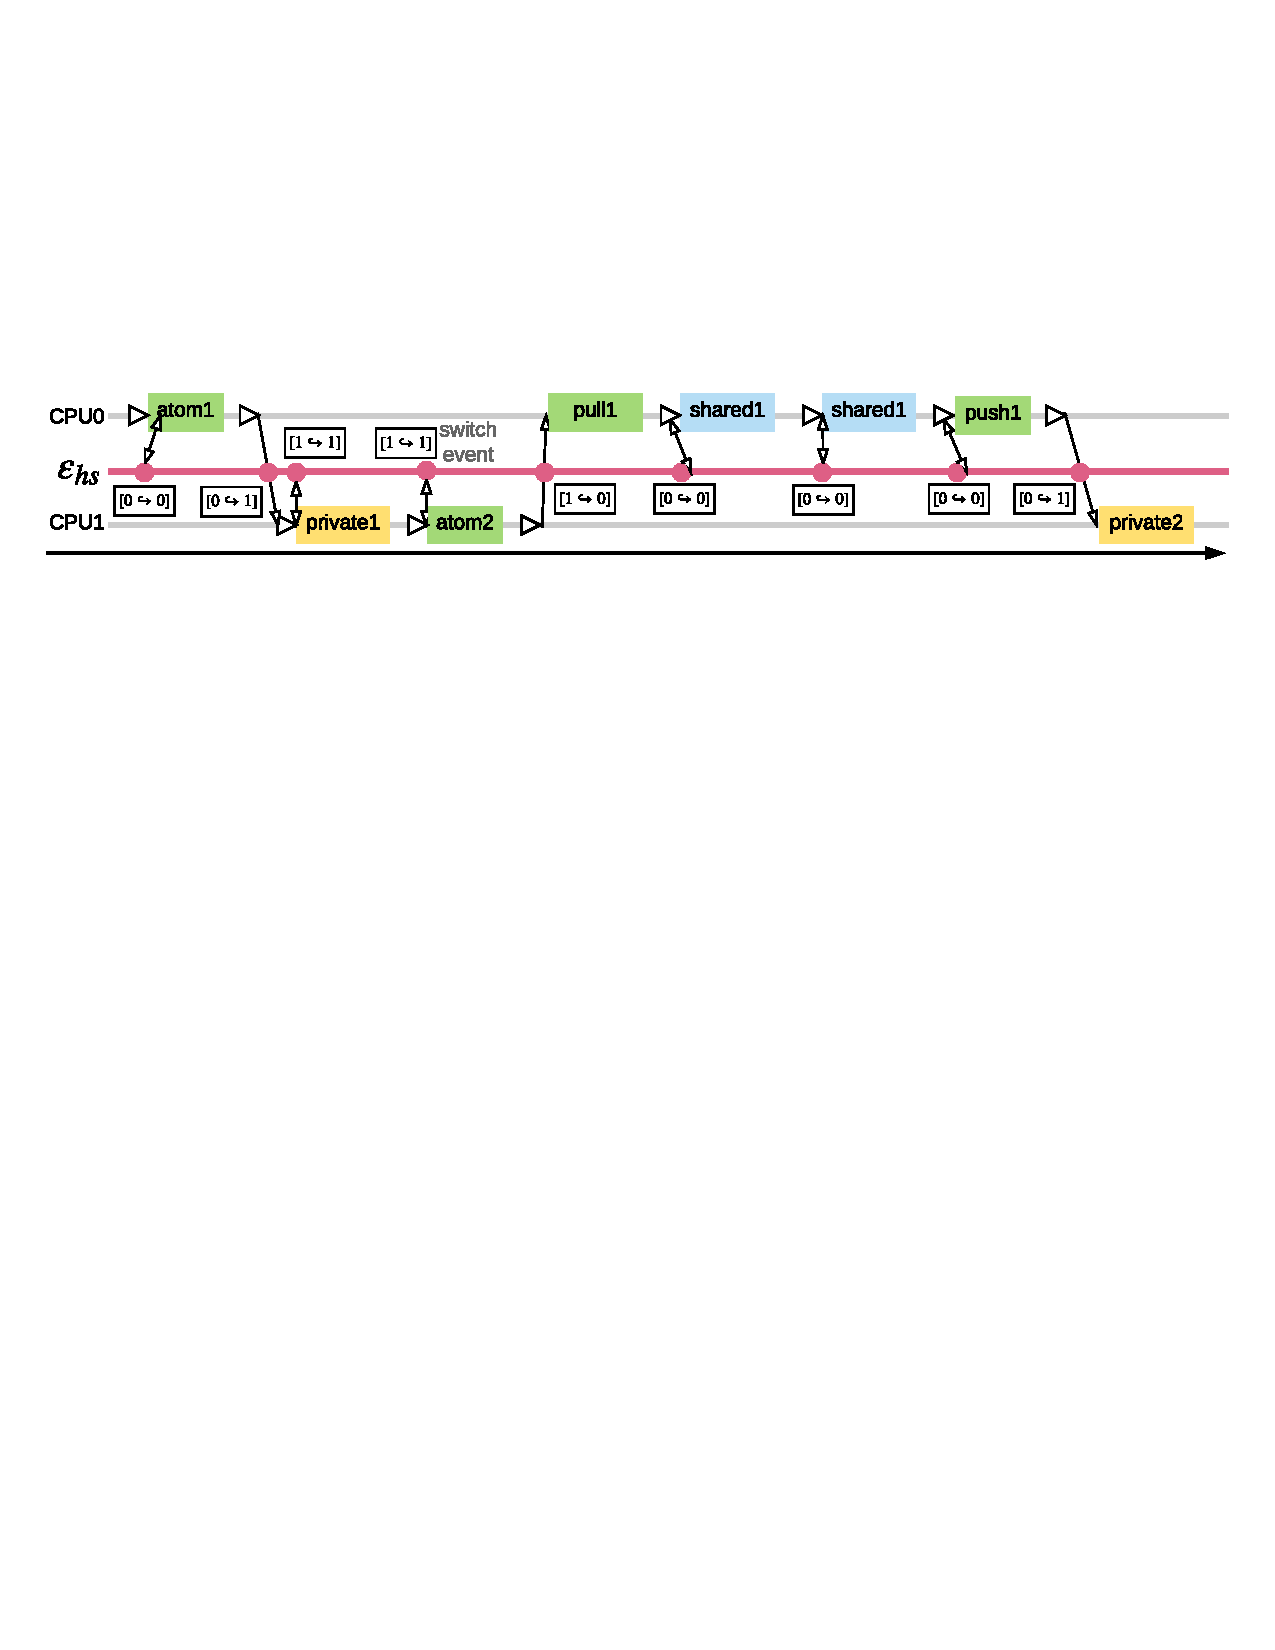
\includegraphics[scale=.52]{figs/machine2}
\vspace{-5pt}
\]

\noindent
The log recorded by this execution is as follows
(a switch from CPU $i$ to $j$ is denoted as $i\switch j$):\vspace{-5pt}
%%%
\[
\begin{footnotesize}
\begin{array}{l}
\!\!\!\!\![\event{0\switch 0, 0.atom_1,  0\switch 1, 1\switch 1,}
\event{1\switch 1, 1.atom_2, 1\switch 0, 0\switch 0,  0\switch 1}]
\end{array}
\end{footnotesize}
\vspace{-5pt}
\]

The behavior of running a program $P$
over this model with a hardware scheduler $\hardoracle$
is denoted as $\mach{hs}(P,\hardoracle)$.
Let $\ectxtc_{hs}$ represents the set of all possible hardware
schedulers. Then we define the whole-machine semantics.
{\small \[
\sem{hs}{P} = \{ ~ \mach{hs}(P,\hardoracle) ~ \mid ~ \hardoracle \in \ectxtc_{hs} ~ \}
\vspace{-15pt}
\]}

\ignore{The machine model with hardware scheduler is denoted as $(\mach{hs}, \hardoracle)$,
to indicate that it is parametrized over all possible $\hardoracle$.}

\noindent
Note that this is a special case of the definition in Sec.~\ref{sec:overview}
for the whole-machine semantics of a concurrent layer machine, where the 
active set is the set of all CPUs.
To ensure correctness of this machine model with respect to the hardware machine model,
we prove that $\mach{x86mc}$ \emph{contextually refines} the new model.
Before we state the property, we first define the notion of
\emph{contextual refinement} formally.

\begin{definition}[Contextual Refinement]
\label{def:mach:refine}
We say layer $L_0$ 
\emph{contextually refines}
layer $L_1$ (written $\forall P, \sem{L_0}{P}\machrel \sem{L_1}{P}$),
iff, for any $P$ that 
does not go wrong 
on $\machx_{L_1}$ under any configuration, (1)~$P$ does not go wrong on $\machx_{L_0}$
under any configuration;
and (2)~any observable behavior of $P$ on $\machx_{L_0}$
under some configuration is also observed on $\machx_{L_1}$
under some (possibly different) configuration.
\end{definition}

\begin{lemma}[Correctness of the hardware scheduler model]\vspace{-3pt}
\label{lemma:hs}
\begin{small}
$$\forall P, \sem{x86mc}{P}\machrel \sem{hs}{P}$$
\end{small}
\vspace{-10px}
\proof[Proof Sketch]
For any interleaved execution on $\machx_{x86mc}$, we construct
a corresponding hardware scheduler on $\mach{hs}$.

\ignore{
Given an observable execution behavior of $P$ running on
$\machx_{x86mc}$, we can construct a particular hardware scheduler
$\hardoracle$ encoding the interleaving that produced the behavior.
The resulting behavior $\mach{hs}(P,\hardoracle)$ is then
an element of $\sem{hs}{P}$ by definition.
}

\ignore{\proof
For any $P$ and any possible interleaving on $\mach{hw}$,
there exists a corresponding hardware scheduler $\hardoracle$,
such that $P$ exhibits an equivalent
behavior when it runs on top of $(\mach{hs}, \hardoracle)$.
\qed}
\end{lemma}

\ignore{
Lemma \ref{lemma:hs} ensures that for
any program running on top of the machine $\mach{hw}$, there exists
a hardware scheduler such that the program exhibits an equivalent
behavior when it runs on top of $\mach{hs}$ with the
hardware scheduler.}

\vspace{-5pt}
\subsection{Machine with local copy of shared memory}
The above machine model does not restrict any access to the shared memory.
We therefore abstract the machine model with hardware scheduler into
a new model that enforces well-synchronized accesses to shared memory.

In addition to the global shared memory concurrently manipulated by all CPUs,
each CPU on this new machine model ($\mach{lcm}$) also maintains
a local copy along with a \emph{valid bit}.
The relation between a CPU's local copy and the global shared memory
is maintained through two new \emph{logical} primitives $\code{pull}$ and $\code{push}$.
The $\code{pull}$ operation updates a CPU's local copy to be equal to the shared memory,
marking the local copy as $\code{valid}$ and the shared memory as $\code{invalid}$.
Conversely, the $\code{push}$ operation updates the shared memory
to be equal to the local copy, marking the shared memory
as $\code{valid}$ and the local copy as $\code{invalid}$.
If a program attempts to pull an $\code{invalid}$ shared memory, push
an $\code{invalid}$ local copy, or access an $\code{invalid}$ local copy,
the program goes wrong.
It makes sure that every shared memory access is always performed on
its $\code{valid}$ local copy, thus systematically enforcing valid accesses to the
shared memory.
Note that all of these constructions are completely \emph{logical}, and do not
correspond to any physical protection mechanisms; thus they do not introduce any
performance overhead.

The shared memory updates of the previous example can be simulated 
on $\mach{lcm}$ as follows:\vspace{-5pt}
\[
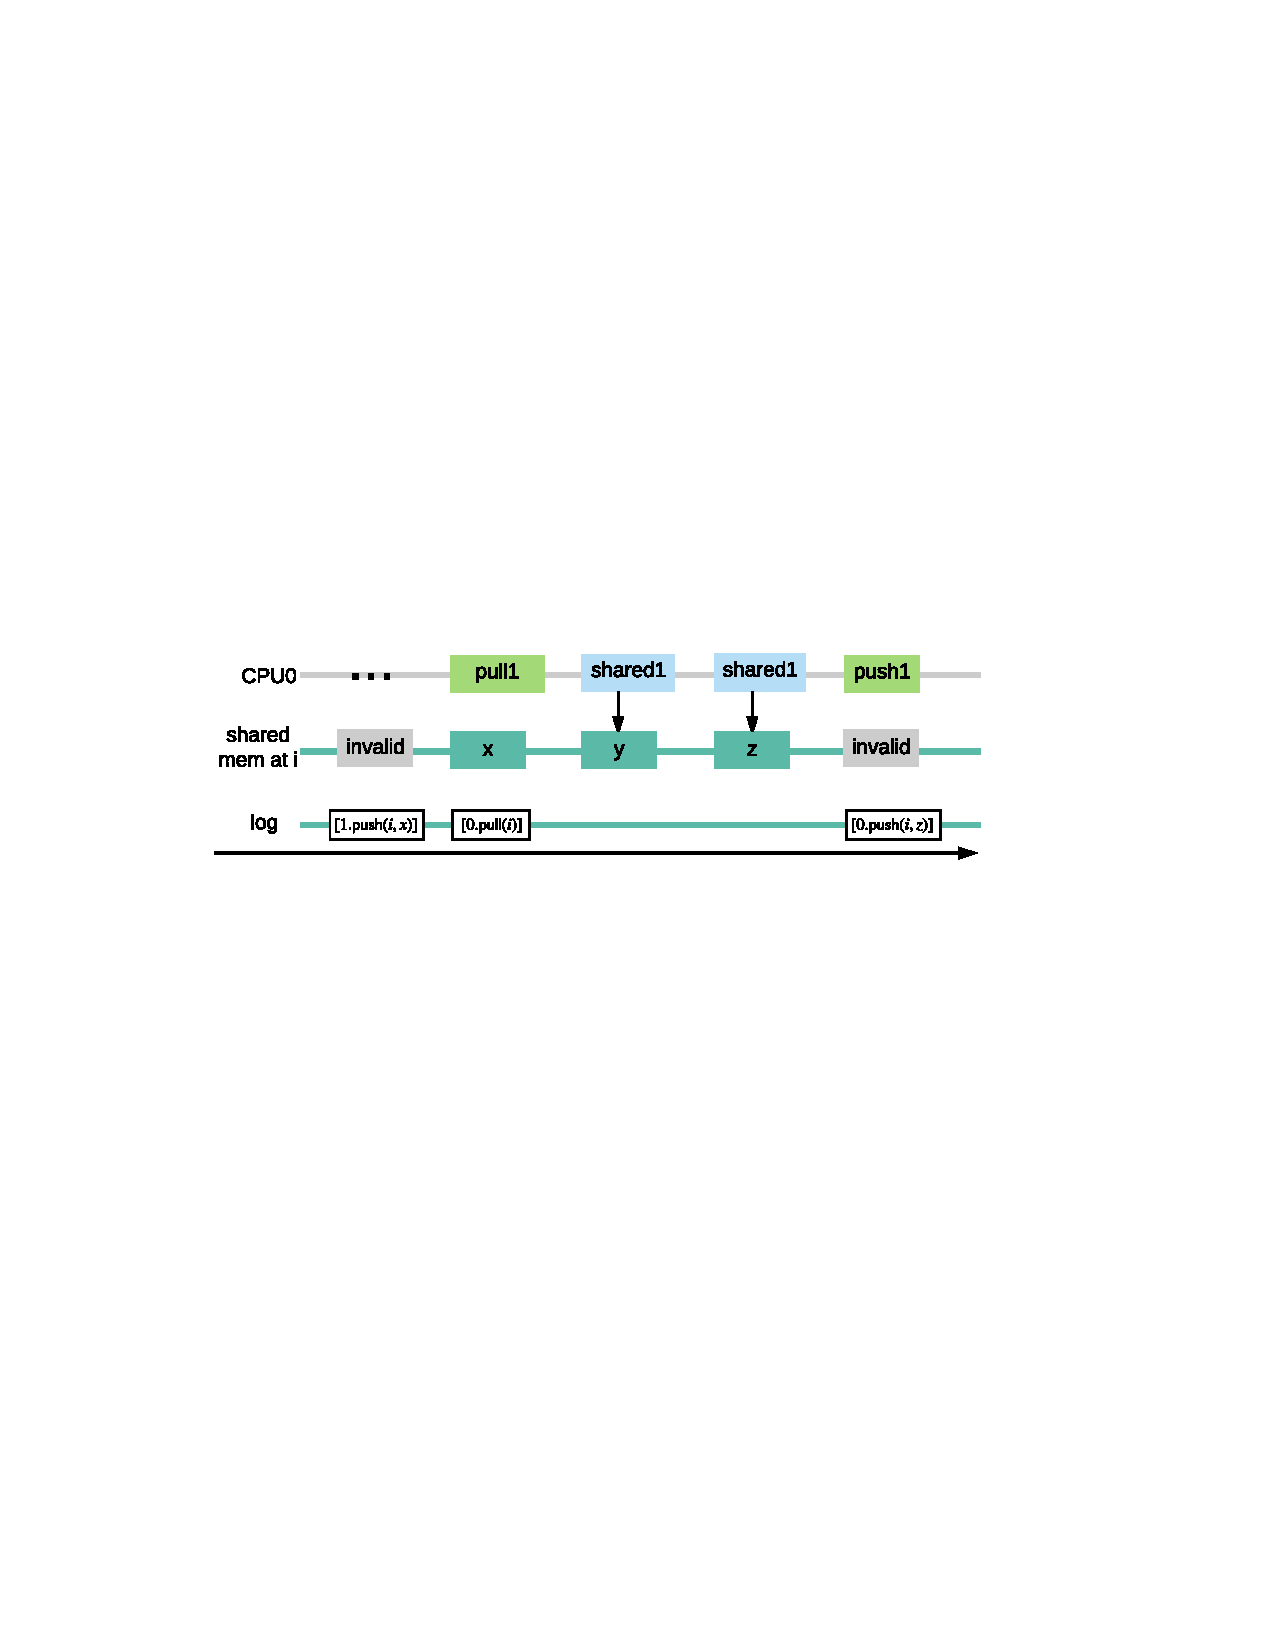
\includegraphics[scale=.6]{figs/machine3}
\vspace{-5pt}
\]

\paragraph{Data-race freedom}
Among the global shared memory and all the local copies, only one can be $\code{valid}$ at any single moment of 
machine execution. 
Therefore, for any program $P$ with a potential \emph{data race}, there exists
a hardware scheduler such that $P$ goes wrong on $\mach{lcm}$.
By showing that a program $P$ is safe (never goes wrong) on $\mach{lcm}$
for \emph{all possible} hardware schedulers, we guarantee that $P$ is data-race free. 

It remains to show that $\mach{lcm}$ is correct with
respect to the previous machine model $\mach{hs}$
with the $\ectxtc_{hs}$.
\begin{lemma}[Correctness of the local copy model]\vspace{-2pt}
{\small \[
\forall P, \sem{hs}{P}\machrel \sem{lcm}{P}\]}
\vspace{-20pt}
%%%
\ignore{
\[\forall \hardoracle, (\mach{hs}, \hardoracle) \machrel 
(\mach{lcm},\hardoracle)\]
}
\ignore{\[\forall P\ \hardoracle, \machbe{P}{\mach{hs}}{\hardoracle}\machrel 
\machbe{P}{\mach{lcm}}{\hardoracle}\]
\proof
For any possible $\hardoracle$, if the program $P$ is safe on $\mach{lcm}$,
then the observable behavior of $P$ on $\mach{lcm}$ is equivalent to
the behavior of $P$ running over $\mach{hs}$.
\qed}
\end{lemma}

\subsection{Partial machine with environment context}

Although $\mach{lcm}$ provides a way to reason about shared memory operations,
it still does not have much support for CPU-local reasoning.
To support modular verification, the machine model should provide
a way to reason about programs on each CPU locally by specifying
expected behaviors of the context programs on other CPUs. The model
should then provide a systematic
way to link the proofs of different local components together to form a global
claim about the whole system. To this purpose, we introduce a partial
machine model $\mach{pt}$ that can be used to reason about the
programs running on a subset of CPUs, by
parametrizing the model over the behaviors of an \emph{environment context}
(\ie, the rest of the CPUs).

We call a given local subset of CPUs the \emph{active CPU set} 
(denoted as $A$).
\ignore{, while all other CPUs are called the 
\emph{context CPU set}.
 of $A$
(denoted as $\overline A$).}
The partial machine model is configured with an active CPU set,
and it queries the environment context whenever it reaches a switch point
that attempts to switch to a CPU outside the active set.

\vspace{-2pt}
\paragraph{Environment context}
of $A$ in this machine model 
is denoted as $\ectxt{pt,A}$.
Each environment context $\oracle_{pt(A)}\in\ectxt{pt,A}$
is a \emph{response function},
which takes the current log 
and returns a list of events from the context programs (\ie, those outside of $A$) 
that is guaranteed to satisfy some invariant.
In other words, response function simulates the observable behavior 
of the context CPUs, and the invariant states the assumptions being 
made over the context.
The hardware scheduler
is also a part of the environment context,
\ie, the events returned by the response function include
switch events. The execution of CPU 0 in the previous example can be simulated
with a $\oracle_{pt(\set{0})}$.
\ignore{$\oracle_{\overline{\set{0}}}$
(\ie, $\oracle_{\set{1}}$, since there are only two CPUs).}\vspace{-2pt}
\[
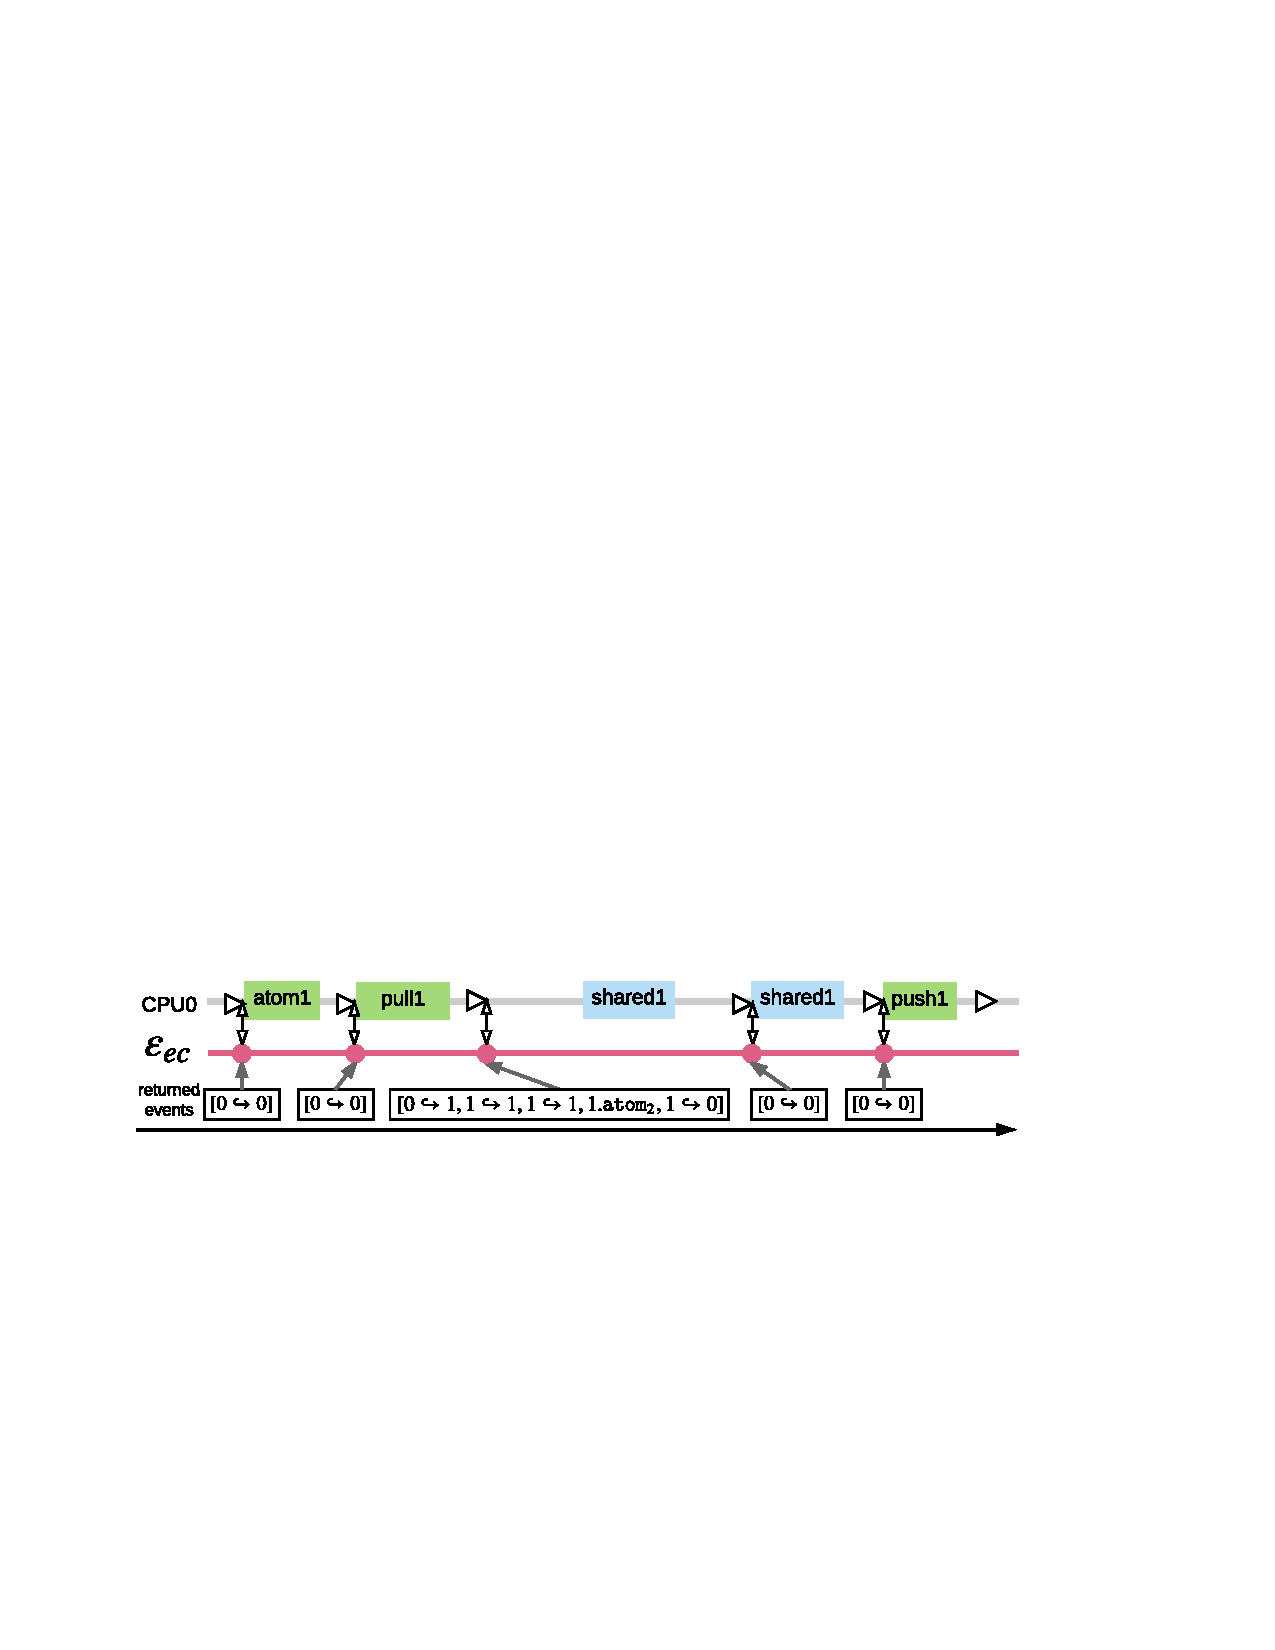
\includegraphics[scale=.53]{figs/machine4}
\vspace{-3pt}
\]

\ignore{The environment context $\oracle_{\set{1}}$
generates the event list $[\event{0\switch 1},\event{1\switch 1},\event{1\switch 1}, \event{1.atom_2}, \event{1\switch 0}]$
at the third \intptext.}

\paragraph{Composition of partial machine models}
Suppose we have verified that two programs, separately running with two 
\emph{disjoint} active CPU sets $A$ and $B$, produce event lists
satisfying invariants $\inv_A$ and $\inv_B$, respectively.
If $\inv_A$ is consistent with the environment context invariant
of $B$,\ignore{(\ie,  $\ectxt{pt,B}$)\ronghui{Do we need this i.e. ?},}
and $\inv_B$ is consistent with the environment context invariant of 
$A$,\ignore{ (\ie, $\ectxt{pt,A}$),}
then we can compose the two separate programs into a single program
with active set $A \cup B$.
This combined program is guaranteed to produce event lists
satisfying the combined invariant $\inv_A \wedge \inv_B$.
Formally, using the whole-machine semantics definition from
Sec.~\ref{sec:overview}, we express this composition as a contextual 
refinement.

\begin{lemma}[Composition of partial machine models]\vspace{-2pt}
\label{lemma:compose}
{\small \[\forall P, \sem{pt(A\cup B)}{P}\machrel \sem{pt(A)}{P} \cap \sem{pt(B)}{P}\quad \text{if } A \cap B = \emptyset\]}
\vspace{-17pt}
\ignore{
\[
\begin{array}{l}
\forall \oracle_{A}\  \oracle_{B}\
\oracle_{\overline{A\cup B}},\\
(\mach{pt},
\oracle_{\overline{A\cup B}})_{A\cup B}
= (\mach{pt},
\oracle_B
\cup \oracle_{\overline{A\cup B}})_A \bigcap
(\mach{pt},
\oracle_A \cup \oracle_{\overline{A\cup B}})_B
\end{array}
\]
}
\ignore{
\proof
If the environment contexts of program $P$ running on $A$ and $B$ are consistent,
then it is equivalent to running $P$ on $A\cup B$ directly. 
\qed}
\end{lemma}

After composing the programs on all CPUs, the context CPU set becomes
empty, and the composed invariant holds on the whole machine.
Since there is no context CPU, the environment context is
reduced to the \emph{hardware scheduler}, which only generates the
switch events. In other words, letting $C$ be the entire set of CPUs
on the machine, we have that $\ectxt{pt,C} = \ectxtc_{hs}$.  By
showing that this \emph{composed machine} with the entire CPU set $C$
is refined by $\mach{lcm}$, the proofs can be propagated down to the
multicore hardware model.

\begin{lemma}[Correctness of the composed total machine]
{\small \[\vspace{-10pt}\forall P, \sem{lcm}{P}\machrel \sem{pt(C)}{P}\vspace{-10pt}\]}
\ignore{
\[
\forall \hardoracle,
(\mach{lcm}, \hardoracle)
\machrel 
(\mach{pt},\hardoracle)\]
}
\ignore{
\[
\forall P\ \hardoracle\ \inv,
\machbe{P}{\mach{lcm}}{\hardoracle}
\machrel 
\machbe{P}{\mach{pt}}{\hardoracle,\inv}\]
\proof
For any given $\hardoracle$, the only difference between two machine models is that
$\mach{partial}$ introduces the invariant $\inv$.
\qed
}
\end{lemma}

\subsection{CPU-local machine model}
\label{subsec:spec:seq}
If we focus on a single active CPU $i$,
the partial machine model is like a \emph{local} machine
with an environment context representing all other CPUs. However,
in this model there is a {\intptext} before each instruction,
so program verification still needs to handle many unnecessary 
interleavings (\eg, the ones between private operations).
In this subsection, we introduce a CPU-local
machine model (denoted as $\mach{loc}$) for a CPU $i$, in which {\intptext}s
only appear before atomic or $\code{push}$/$\code{pull}$ operations.
The {\intptext}s before shared or private operations
are removed via two steps: \emph{shuffling} and \emph{merging}.

\paragraph{Shuffling {\intptext}s}
In $\mach{loc}$, we introduce a \emph{log cache}~--- for
the {\intptext}s before shared and private operations,
the query results from the environment context
are stored in a temporary log cache.
The cached events are applied to the logical log
just before the next atomic or $\code{push}$/$\code{pull}$ operation.
Thus, when we perform shared or private operations,
the observations of the environment context are delayed
until the next atomic or $\code{push}$/$\code{pull}$ operation.
This is possible because a shared operation can only be performed
when the current local copy of shared memory is valid, meaning that 
no other context program can interfere with the operation.

\paragraph{Merging {\intptext}s} Once the {\intptext}s are shuffled properly,
we merge all the adjacent {\intptext}s together.
When we merge {\intptext}s, we also need to merge 
the switch events generated by the environment context.
For example, the change of {\intptext}s for the previous example
on CPU-local machine is as follows: 
\[
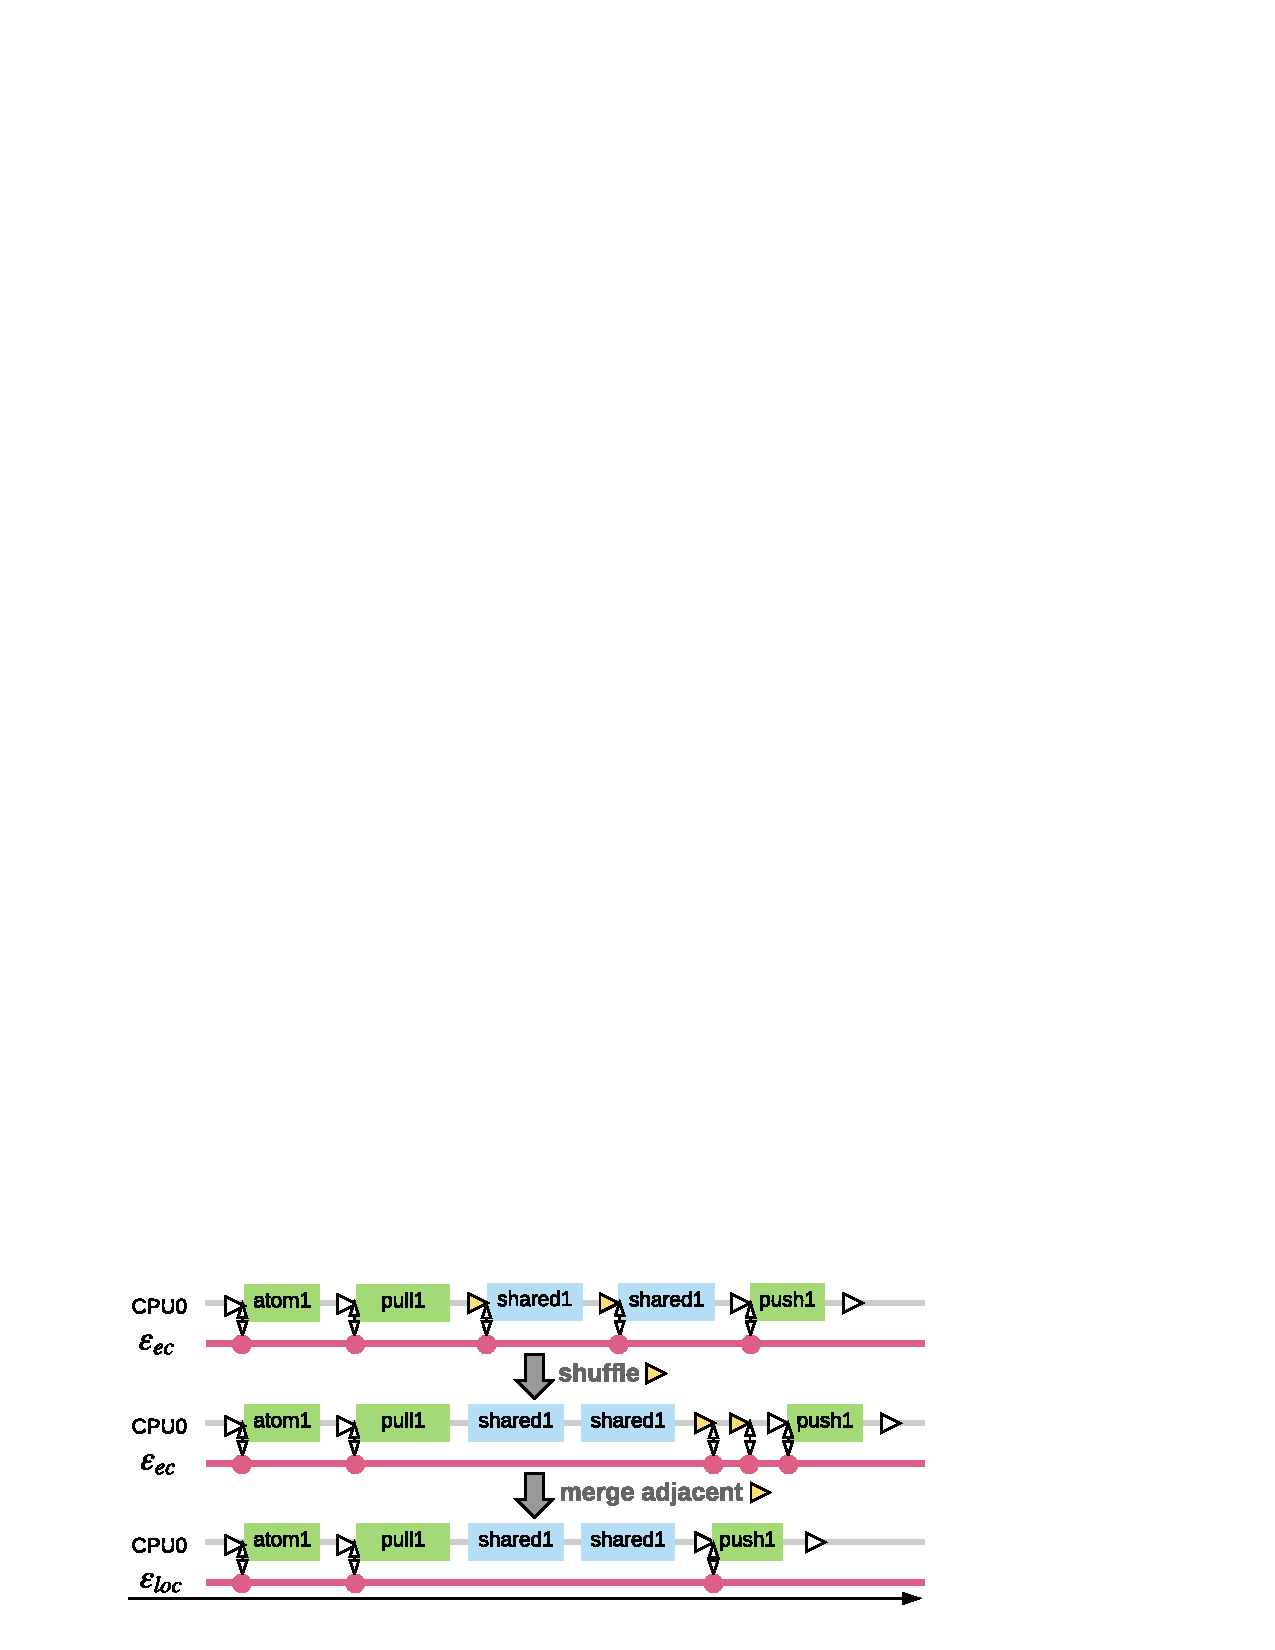
\includegraphics[scale=.57]{figs/machine5}
\]

\begin{lemma}[Correctness of CPU-local machine model]
{\small \[\forall P, \sem{pt(\set{i})}{P}\machrel \sem{loc(\set{i})}{P}\]}
\vspace{-23pt}

\ignore{
\[
\forall \oracle_{\overline{\set{i}}},
\exists \oracle'_{\overline{\set{i}}},
(\mach{pt},\oracle_{\overline{\set{i}}})_{\set{i}}
\machrel 
(\mach{loc},\oracle'_{\overline{\set{i}}})_{\set{i}}
\]
}
\ignore{\[
\begin{array}{l}
\forall P\ \oracle_{\overline{\set{i}}}\ \inv_{\set{i}},
\exists \oracle'_{\overline{\set{i}}},\\
\machbe{P}{\mach{pt}}{\oracle_{\overline{\set{i}}},  \inv_{\set{i}}}
\machrel 
\machbe{P}{\mach{loc}}{\oracle'_{\overline{\set{i}}}, \inv_{\set{i}}}
\end{array}
\]
\proof
Shuffling and merging {\intptext}s  are valid.
\qed}
\end{lemma}

Finally, we obtain the refinement relation from the multicore
hardware model
to the CPU-local machine model by composing
all of the refinement relations together (\cf Fig.~\ref{fig:spec:chain}).
We introduce and verify the {\mCTOS} kernel on top of the CPU-local machine
model $\mach{loc}$. The refinement proof guarantees that the proved properties can be
propagated down to the multicore hardware model $\mach{x86mc}$.





\ignore{
\newman{Copied from the overview section. I will merge them into this
section somehow.}
\subsection{Defining abstraction layers}

We define a concurrent
layer interface $L$ using three components: a collection of
\emph{private objects}, a collection of \emph{atomic objects}, and the
invariants which the atomic and private objects must satisfy at any
point of the execution.  These three components define a {\em logical}
view of a subset of the kernel code and extend an x86-like assembly
machine ($\machx$) with an abstract specification of that code. 

A {\em private object} is the abstraction of private date owned by a
particular thread (or process or CPU). It consists of an
\emph{abstract state} (serving as the abstraction of the underlying
private memory), and a collection of primitives (serving as the
specifications of the methods manipulating that piece of the private
memory). Fig.~\ref{fig:spec:object} shows how to build private
objects.

An {\em atomic object} is the abstraction of shared memory. All of
its methods/primitives are atomic.

As shown in Sec.XXX, the sequential machine model contains a
\emph{small} set of atomic objects, which generates a single event and
the object itself is constructable by replaying the logical log.

Figure~\ref{fig:spec:object} shows how to build atomic objects based
on the atomic objects, private objects, and the shared memory at
underlay.  Since the shared memory accesses are modeled using
\emph{local copy}, the \code{push/pull} operations have to be
synchronized using underlay's atomic objects.  The verification of
functions accessing shared data inside the kernel is a procedure to
show that all shared memory accesses are well-synchronized and its
invocation can be viewed as atomic.

For example, the physical page allocator scans the \emph{shared}
allocation table and returns the first free page.  Its accesses to the
shared table are protected by \emph{atomic lock objects}, such that
its \code{push/pull} operations are safe to execute.  By showing that
the allocator implementation satisfy the specification, which
generates a single \code{palloc} event, an atomic allocator object is
introduced and can be used to reason about other kernel modules at
higher layers (\cf Sec.\ref{sec:base:memm}).

We will use $\mach{L}$ to denote the resulting abstract machine for
each layer interface $L$





\paragraph{Layer invariant}
Each abstraction layer specifies a predicate
on the private objects' abstract states
and the logical log,
which is the invariant $\inv_{\set{i}}$ hold for the execution on CPU $i$
(\cf Sec.XXX).
We have to show that this invariant $\inv_{\set{i}}$ is preserved
by all primitives of private objects and atomic objects.
The proofs for atomic  objects also rely on the
invariant of the context CPUs (\ie, $\inv_{\bar{\set{i}}}$).

In previous verification efforts, even for private objects,
proving invariants has typically been challenging~\cite{klein2009sel4},
especially that the invariants might be temporarily violated within the function body.
For example, adding a new node to a doubly-linked list
temporarily violates invariants that the list is well formed.

However, in our layered approach,
we do not have to set up the all the invariants at a single step.
Take the thread queue (implemented as doubly-linked list) in C2 kernel as an example.
When verifying the concrete implementation, we do not pose the well-formedness invariant
over the queue at that layer.
We only prove the invariant after the queue and its operations be introduced as a private object and the primitives.
In this way,
since the abstract primitives are atomic,
there is no longer a point in the execution
at which the invariants have to be temporarily violated.




\subsection{Contextual Refinement}
The contextual refinement relation between
the two layers (one with concrete implementation and the other
with the private and atomic object) ensures that any kernel/user context code 
(\ie, threads on other CPUs and other modules on the same CPU)
linking with the more abstract layer retains an
equivalent behavior when linking with the corresponding
concrete implementation running on the layer.

\paragraph{Contextual refinement for private objects}
As shown in Fig.~\ref{fig:spec:object},
to establish the contextual refinement relation
between concrete memory and the private object,
we use memory permissions~\cite{leroy08} at the higher layer
to prevent the context code
from accessing the private memory.
Note that these permissions do \emph{not}
correspond to a physical protection mechanism,
but instead are entirely logical:
they ensure that the higher-level abstract machine
gets stuck whenever it executes
code that directly accesses this private memory without going through the provided
primitives. By proving that our kernel is safe (it will not go wrong),
we guarantee that this situation will not happen.

\paragraph{Contextual refinement for atomic objects}
To establish the contextual refinement relation
for atomic objects, the main proof body is about the invariants proof.
We have to show that for any environment context $\oracle_{\bar{\set{i}}}$
that satisfy the context invariant $\inv_{\bar{\set{i}}}$.
Thus, the environment context linked with CPU $i$'s atomic object
is equivalent to the one linked with the concrete implementation,
where interleaving might happen within the function body.

\paragraph{Layer refinement}


The first layer \emph{PreInit} (\ie, $L_0$)
is based on the \emph{sequential machine model} $\mach{s}$.
As shown in Fig.\ref{fig:spec:refine_layer},
kernel modules
are verified as a stack of layers
building 
on top of the $\mach{s}$.
Although the layers are built
on behave of a particular $\text{CPU}_i$,
layers at other CPUs are symmetric.
After the scheduler module is verified,
we move one step forward
and decompose the execution on $\text{CPU}_i$
into a collection of \emph{per-thread execution}.
By introducing the \emph{software scheduler}
$\oracle_{ss}$ (\ie, reflecting the scheduling algorithm),
multi-threads execution on the same CPU 
can be composed similarly to the multi-core composition
(\cf Sec.~\ref{sec:base:procm}).
Thus, user programs can be verified
locally using the atomic specifications of kernel's
system calls,
and be composed using our framework.

}


     % Concurrent Abstraction Layers (1.5 pages)

